\documentclass[11pt]{article}

    \usepackage[breakable]{tcolorbox}
    \usepackage{parskip} % Stop auto-indenting (to mimic markdown behaviour)
    
    \usepackage{iftex}
    \ifPDFTeX
    	\usepackage[T1]{fontenc}
    	\usepackage{mathpazo}
    \else
    	\usepackage{fontspec}
    \fi

    % Basic figure setup, for now with no caption control since it's done
    % automatically by Pandoc (which extracts ![](path) syntax from Markdown).
    \usepackage{graphicx}
    % Maintain compatibility with old templates. Remove in nbconvert 6.0
    \let\Oldincludegraphics\includegraphics
    % Ensure that by default, figures have no caption (until we provide a
    % proper Figure object with a Caption API and a way to capture that
    % in the conversion process - todo).
    \usepackage{caption}
    \DeclareCaptionFormat{nocaption}{}
    \captionsetup{format=nocaption,aboveskip=0pt,belowskip=0pt}

    \usepackage[Export]{adjustbox} % Used to constrain images to a maximum size
    \adjustboxset{max size={0.9\linewidth}{0.9\paperheight}}
    \usepackage{float}
    \floatplacement{figure}{H} % forces figures to be placed at the correct location
    \usepackage{xcolor} % Allow colors to be defined
    \usepackage{enumerate} % Needed for markdown enumerations to work
    \usepackage{geometry} % Used to adjust the document margins
    \usepackage{amsmath} % Equations
    \usepackage{amssymb} % Equations
    \usepackage{textcomp} % defines textquotesingle
    % Hack from http://tex.stackexchange.com/a/47451/13684:
    \AtBeginDocument{%
        \def\PYZsq{\textquotesingle}% Upright quotes in Pygmentized code
    }
    \usepackage{upquote} % Upright quotes for verbatim code
    \usepackage{eurosym} % defines \euro
    \usepackage[mathletters]{ucs} % Extended unicode (utf-8) support
    \usepackage{fancyvrb} % verbatim replacement that allows latex
    \usepackage{grffile} % extends the file name processing of package graphics 
                         % to support a larger range
    \makeatletter % fix for grffile with XeLaTeX
    \def\Gread@@xetex#1{%
      \IfFileExists{"\Gin@base".bb}%
      {\Gread@eps{\Gin@base.bb}}%
      {\Gread@@xetex@aux#1}%
    }
    \makeatother

    % The hyperref package gives us a pdf with properly built
    % internal navigation ('pdf bookmarks' for the table of contents,
    % internal cross-reference links, web links for URLs, etc.)
    \usepackage{hyperref}
    % The default LaTeX title has an obnoxious amount of whitespace. By default,
    % titling removes some of it. It also provides customization options.
    \usepackage{titling}
    \usepackage{longtable} % longtable support required by pandoc >1.10
    \usepackage{booktabs}  % table support for pandoc > 1.12.2
    \usepackage[inline]{enumitem} % IRkernel/repr support (it uses the enumerate* environment)
    \usepackage[normalem]{ulem} % ulem is needed to support strikethroughs (\sout)
                                % normalem makes italics be italics, not underlines
    \usepackage{mathrsfs}
    

    
    % Colors for the hyperref package
    \definecolor{urlcolor}{rgb}{0,.145,.698}
    \definecolor{linkcolor}{rgb}{.71,0.21,0.01}
    \definecolor{citecolor}{rgb}{.12,.54,.11}

    % ANSI colors
    \definecolor{ansi-black}{HTML}{3E424D}
    \definecolor{ansi-black-intense}{HTML}{282C36}
    \definecolor{ansi-red}{HTML}{E75C58}
    \definecolor{ansi-red-intense}{HTML}{B22B31}
    \definecolor{ansi-green}{HTML}{00A250}
    \definecolor{ansi-green-intense}{HTML}{007427}
    \definecolor{ansi-yellow}{HTML}{DDB62B}
    \definecolor{ansi-yellow-intense}{HTML}{B27D12}
    \definecolor{ansi-blue}{HTML}{208FFB}
    \definecolor{ansi-blue-intense}{HTML}{0065CA}
    \definecolor{ansi-magenta}{HTML}{D160C4}
    \definecolor{ansi-magenta-intense}{HTML}{A03196}
    \definecolor{ansi-cyan}{HTML}{60C6C8}
    \definecolor{ansi-cyan-intense}{HTML}{258F8F}
    \definecolor{ansi-white}{HTML}{C5C1B4}
    \definecolor{ansi-white-intense}{HTML}{A1A6B2}
    \definecolor{ansi-default-inverse-fg}{HTML}{FFFFFF}
    \definecolor{ansi-default-inverse-bg}{HTML}{000000}

    % commands and environments needed by pandoc snippets
    % extracted from the output of `pandoc -s`
    \providecommand{\tightlist}{%
      \setlength{\itemsep}{0pt}\setlength{\parskip}{0pt}}
    \DefineVerbatimEnvironment{Highlighting}{Verbatim}{commandchars=\\\{\}}
    % Add ',fontsize=\small' for more characters per line
    \newenvironment{Shaded}{}{}
    \newcommand{\KeywordTok}[1]{\textcolor[rgb]{0.00,0.44,0.13}{\textbf{{#1}}}}
    \newcommand{\DataTypeTok}[1]{\textcolor[rgb]{0.56,0.13,0.00}{{#1}}}
    \newcommand{\DecValTok}[1]{\textcolor[rgb]{0.25,0.63,0.44}{{#1}}}
    \newcommand{\BaseNTok}[1]{\textcolor[rgb]{0.25,0.63,0.44}{{#1}}}
    \newcommand{\FloatTok}[1]{\textcolor[rgb]{0.25,0.63,0.44}{{#1}}}
    \newcommand{\CharTok}[1]{\textcolor[rgb]{0.25,0.44,0.63}{{#1}}}
    \newcommand{\StringTok}[1]{\textcolor[rgb]{0.25,0.44,0.63}{{#1}}}
    \newcommand{\CommentTok}[1]{\textcolor[rgb]{0.38,0.63,0.69}{\textit{{#1}}}}
    \newcommand{\OtherTok}[1]{\textcolor[rgb]{0.00,0.44,0.13}{{#1}}}
    \newcommand{\AlertTok}[1]{\textcolor[rgb]{1.00,0.00,0.00}{\textbf{{#1}}}}
    \newcommand{\FunctionTok}[1]{\textcolor[rgb]{0.02,0.16,0.49}{{#1}}}
    \newcommand{\RegionMarkerTok}[1]{{#1}}
    \newcommand{\ErrorTok}[1]{\textcolor[rgb]{1.00,0.00,0.00}{\textbf{{#1}}}}
    \newcommand{\NormalTok}[1]{{#1}}
    
    % Additional commands for more recent versions of Pandoc
    \newcommand{\ConstantTok}[1]{\textcolor[rgb]{0.53,0.00,0.00}{{#1}}}
    \newcommand{\SpecialCharTok}[1]{\textcolor[rgb]{0.25,0.44,0.63}{{#1}}}
    \newcommand{\VerbatimStringTok}[1]{\textcolor[rgb]{0.25,0.44,0.63}{{#1}}}
    \newcommand{\SpecialStringTok}[1]{\textcolor[rgb]{0.73,0.40,0.53}{{#1}}}
    \newcommand{\ImportTok}[1]{{#1}}
    \newcommand{\DocumentationTok}[1]{\textcolor[rgb]{0.73,0.13,0.13}{\textit{{#1}}}}
    \newcommand{\AnnotationTok}[1]{\textcolor[rgb]{0.38,0.63,0.69}{\textbf{\textit{{#1}}}}}
    \newcommand{\CommentVarTok}[1]{\textcolor[rgb]{0.38,0.63,0.69}{\textbf{\textit{{#1}}}}}
    \newcommand{\VariableTok}[1]{\textcolor[rgb]{0.10,0.09,0.49}{{#1}}}
    \newcommand{\ControlFlowTok}[1]{\textcolor[rgb]{0.00,0.44,0.13}{\textbf{{#1}}}}
    \newcommand{\OperatorTok}[1]{\textcolor[rgb]{0.40,0.40,0.40}{{#1}}}
    \newcommand{\BuiltInTok}[1]{{#1}}
    \newcommand{\ExtensionTok}[1]{{#1}}
    \newcommand{\PreprocessorTok}[1]{\textcolor[rgb]{0.74,0.48,0.00}{{#1}}}
    \newcommand{\AttributeTok}[1]{\textcolor[rgb]{0.49,0.56,0.16}{{#1}}}
    \newcommand{\InformationTok}[1]{\textcolor[rgb]{0.38,0.63,0.69}{\textbf{\textit{{#1}}}}}
    \newcommand{\WarningTok}[1]{\textcolor[rgb]{0.38,0.63,0.69}{\textbf{\textit{{#1}}}}}
    
    
    % Define a nice break command that doesn't care if a line doesn't already
    % exist.
    \def\br{\hspace*{\fill} \\* }
    % Math Jax compatibility definitions
    \def\gt{>}
    \def\lt{<}
    \let\Oldtex\TeX
    \let\Oldlatex\LaTeX
    \renewcommand{\TeX}{\textrm{\Oldtex}}
    \renewcommand{\LaTeX}{\textrm{\Oldlatex}}
    % Document parameters
    % Document title
    \title{2021\_01\_20\_EE538\_Lecture3\_W2021}
    
    
    
    
    
% Pygments definitions
\makeatletter
\def\PY@reset{\let\PY@it=\relax \let\PY@bf=\relax%
    \let\PY@ul=\relax \let\PY@tc=\relax%
    \let\PY@bc=\relax \let\PY@ff=\relax}
\def\PY@tok#1{\csname PY@tok@#1\endcsname}
\def\PY@toks#1+{\ifx\relax#1\empty\else%
    \PY@tok{#1}\expandafter\PY@toks\fi}
\def\PY@do#1{\PY@bc{\PY@tc{\PY@ul{%
    \PY@it{\PY@bf{\PY@ff{#1}}}}}}}
\def\PY#1#2{\PY@reset\PY@toks#1+\relax+\PY@do{#2}}

\expandafter\def\csname PY@tok@w\endcsname{\def\PY@tc##1{\textcolor[rgb]{0.73,0.73,0.73}{##1}}}
\expandafter\def\csname PY@tok@c\endcsname{\let\PY@it=\textit\def\PY@tc##1{\textcolor[rgb]{0.25,0.50,0.50}{##1}}}
\expandafter\def\csname PY@tok@cp\endcsname{\def\PY@tc##1{\textcolor[rgb]{0.74,0.48,0.00}{##1}}}
\expandafter\def\csname PY@tok@k\endcsname{\let\PY@bf=\textbf\def\PY@tc##1{\textcolor[rgb]{0.00,0.50,0.00}{##1}}}
\expandafter\def\csname PY@tok@kp\endcsname{\def\PY@tc##1{\textcolor[rgb]{0.00,0.50,0.00}{##1}}}
\expandafter\def\csname PY@tok@kt\endcsname{\def\PY@tc##1{\textcolor[rgb]{0.69,0.00,0.25}{##1}}}
\expandafter\def\csname PY@tok@o\endcsname{\def\PY@tc##1{\textcolor[rgb]{0.40,0.40,0.40}{##1}}}
\expandafter\def\csname PY@tok@ow\endcsname{\let\PY@bf=\textbf\def\PY@tc##1{\textcolor[rgb]{0.67,0.13,1.00}{##1}}}
\expandafter\def\csname PY@tok@nb\endcsname{\def\PY@tc##1{\textcolor[rgb]{0.00,0.50,0.00}{##1}}}
\expandafter\def\csname PY@tok@nf\endcsname{\def\PY@tc##1{\textcolor[rgb]{0.00,0.00,1.00}{##1}}}
\expandafter\def\csname PY@tok@nc\endcsname{\let\PY@bf=\textbf\def\PY@tc##1{\textcolor[rgb]{0.00,0.00,1.00}{##1}}}
\expandafter\def\csname PY@tok@nn\endcsname{\let\PY@bf=\textbf\def\PY@tc##1{\textcolor[rgb]{0.00,0.00,1.00}{##1}}}
\expandafter\def\csname PY@tok@ne\endcsname{\let\PY@bf=\textbf\def\PY@tc##1{\textcolor[rgb]{0.82,0.25,0.23}{##1}}}
\expandafter\def\csname PY@tok@nv\endcsname{\def\PY@tc##1{\textcolor[rgb]{0.10,0.09,0.49}{##1}}}
\expandafter\def\csname PY@tok@no\endcsname{\def\PY@tc##1{\textcolor[rgb]{0.53,0.00,0.00}{##1}}}
\expandafter\def\csname PY@tok@nl\endcsname{\def\PY@tc##1{\textcolor[rgb]{0.63,0.63,0.00}{##1}}}
\expandafter\def\csname PY@tok@ni\endcsname{\let\PY@bf=\textbf\def\PY@tc##1{\textcolor[rgb]{0.60,0.60,0.60}{##1}}}
\expandafter\def\csname PY@tok@na\endcsname{\def\PY@tc##1{\textcolor[rgb]{0.49,0.56,0.16}{##1}}}
\expandafter\def\csname PY@tok@nt\endcsname{\let\PY@bf=\textbf\def\PY@tc##1{\textcolor[rgb]{0.00,0.50,0.00}{##1}}}
\expandafter\def\csname PY@tok@nd\endcsname{\def\PY@tc##1{\textcolor[rgb]{0.67,0.13,1.00}{##1}}}
\expandafter\def\csname PY@tok@s\endcsname{\def\PY@tc##1{\textcolor[rgb]{0.73,0.13,0.13}{##1}}}
\expandafter\def\csname PY@tok@sd\endcsname{\let\PY@it=\textit\def\PY@tc##1{\textcolor[rgb]{0.73,0.13,0.13}{##1}}}
\expandafter\def\csname PY@tok@si\endcsname{\let\PY@bf=\textbf\def\PY@tc##1{\textcolor[rgb]{0.73,0.40,0.53}{##1}}}
\expandafter\def\csname PY@tok@se\endcsname{\let\PY@bf=\textbf\def\PY@tc##1{\textcolor[rgb]{0.73,0.40,0.13}{##1}}}
\expandafter\def\csname PY@tok@sr\endcsname{\def\PY@tc##1{\textcolor[rgb]{0.73,0.40,0.53}{##1}}}
\expandafter\def\csname PY@tok@ss\endcsname{\def\PY@tc##1{\textcolor[rgb]{0.10,0.09,0.49}{##1}}}
\expandafter\def\csname PY@tok@sx\endcsname{\def\PY@tc##1{\textcolor[rgb]{0.00,0.50,0.00}{##1}}}
\expandafter\def\csname PY@tok@m\endcsname{\def\PY@tc##1{\textcolor[rgb]{0.40,0.40,0.40}{##1}}}
\expandafter\def\csname PY@tok@gh\endcsname{\let\PY@bf=\textbf\def\PY@tc##1{\textcolor[rgb]{0.00,0.00,0.50}{##1}}}
\expandafter\def\csname PY@tok@gu\endcsname{\let\PY@bf=\textbf\def\PY@tc##1{\textcolor[rgb]{0.50,0.00,0.50}{##1}}}
\expandafter\def\csname PY@tok@gd\endcsname{\def\PY@tc##1{\textcolor[rgb]{0.63,0.00,0.00}{##1}}}
\expandafter\def\csname PY@tok@gi\endcsname{\def\PY@tc##1{\textcolor[rgb]{0.00,0.63,0.00}{##1}}}
\expandafter\def\csname PY@tok@gr\endcsname{\def\PY@tc##1{\textcolor[rgb]{1.00,0.00,0.00}{##1}}}
\expandafter\def\csname PY@tok@ge\endcsname{\let\PY@it=\textit}
\expandafter\def\csname PY@tok@gs\endcsname{\let\PY@bf=\textbf}
\expandafter\def\csname PY@tok@gp\endcsname{\let\PY@bf=\textbf\def\PY@tc##1{\textcolor[rgb]{0.00,0.00,0.50}{##1}}}
\expandafter\def\csname PY@tok@go\endcsname{\def\PY@tc##1{\textcolor[rgb]{0.53,0.53,0.53}{##1}}}
\expandafter\def\csname PY@tok@gt\endcsname{\def\PY@tc##1{\textcolor[rgb]{0.00,0.27,0.87}{##1}}}
\expandafter\def\csname PY@tok@err\endcsname{\def\PY@bc##1{\setlength{\fboxsep}{0pt}\fcolorbox[rgb]{1.00,0.00,0.00}{1,1,1}{\strut ##1}}}
\expandafter\def\csname PY@tok@kc\endcsname{\let\PY@bf=\textbf\def\PY@tc##1{\textcolor[rgb]{0.00,0.50,0.00}{##1}}}
\expandafter\def\csname PY@tok@kd\endcsname{\let\PY@bf=\textbf\def\PY@tc##1{\textcolor[rgb]{0.00,0.50,0.00}{##1}}}
\expandafter\def\csname PY@tok@kn\endcsname{\let\PY@bf=\textbf\def\PY@tc##1{\textcolor[rgb]{0.00,0.50,0.00}{##1}}}
\expandafter\def\csname PY@tok@kr\endcsname{\let\PY@bf=\textbf\def\PY@tc##1{\textcolor[rgb]{0.00,0.50,0.00}{##1}}}
\expandafter\def\csname PY@tok@bp\endcsname{\def\PY@tc##1{\textcolor[rgb]{0.00,0.50,0.00}{##1}}}
\expandafter\def\csname PY@tok@fm\endcsname{\def\PY@tc##1{\textcolor[rgb]{0.00,0.00,1.00}{##1}}}
\expandafter\def\csname PY@tok@vc\endcsname{\def\PY@tc##1{\textcolor[rgb]{0.10,0.09,0.49}{##1}}}
\expandafter\def\csname PY@tok@vg\endcsname{\def\PY@tc##1{\textcolor[rgb]{0.10,0.09,0.49}{##1}}}
\expandafter\def\csname PY@tok@vi\endcsname{\def\PY@tc##1{\textcolor[rgb]{0.10,0.09,0.49}{##1}}}
\expandafter\def\csname PY@tok@vm\endcsname{\def\PY@tc##1{\textcolor[rgb]{0.10,0.09,0.49}{##1}}}
\expandafter\def\csname PY@tok@sa\endcsname{\def\PY@tc##1{\textcolor[rgb]{0.73,0.13,0.13}{##1}}}
\expandafter\def\csname PY@tok@sb\endcsname{\def\PY@tc##1{\textcolor[rgb]{0.73,0.13,0.13}{##1}}}
\expandafter\def\csname PY@tok@sc\endcsname{\def\PY@tc##1{\textcolor[rgb]{0.73,0.13,0.13}{##1}}}
\expandafter\def\csname PY@tok@dl\endcsname{\def\PY@tc##1{\textcolor[rgb]{0.73,0.13,0.13}{##1}}}
\expandafter\def\csname PY@tok@s2\endcsname{\def\PY@tc##1{\textcolor[rgb]{0.73,0.13,0.13}{##1}}}
\expandafter\def\csname PY@tok@sh\endcsname{\def\PY@tc##1{\textcolor[rgb]{0.73,0.13,0.13}{##1}}}
\expandafter\def\csname PY@tok@s1\endcsname{\def\PY@tc##1{\textcolor[rgb]{0.73,0.13,0.13}{##1}}}
\expandafter\def\csname PY@tok@mb\endcsname{\def\PY@tc##1{\textcolor[rgb]{0.40,0.40,0.40}{##1}}}
\expandafter\def\csname PY@tok@mf\endcsname{\def\PY@tc##1{\textcolor[rgb]{0.40,0.40,0.40}{##1}}}
\expandafter\def\csname PY@tok@mh\endcsname{\def\PY@tc##1{\textcolor[rgb]{0.40,0.40,0.40}{##1}}}
\expandafter\def\csname PY@tok@mi\endcsname{\def\PY@tc##1{\textcolor[rgb]{0.40,0.40,0.40}{##1}}}
\expandafter\def\csname PY@tok@il\endcsname{\def\PY@tc##1{\textcolor[rgb]{0.40,0.40,0.40}{##1}}}
\expandafter\def\csname PY@tok@mo\endcsname{\def\PY@tc##1{\textcolor[rgb]{0.40,0.40,0.40}{##1}}}
\expandafter\def\csname PY@tok@ch\endcsname{\let\PY@it=\textit\def\PY@tc##1{\textcolor[rgb]{0.25,0.50,0.50}{##1}}}
\expandafter\def\csname PY@tok@cm\endcsname{\let\PY@it=\textit\def\PY@tc##1{\textcolor[rgb]{0.25,0.50,0.50}{##1}}}
\expandafter\def\csname PY@tok@cpf\endcsname{\let\PY@it=\textit\def\PY@tc##1{\textcolor[rgb]{0.25,0.50,0.50}{##1}}}
\expandafter\def\csname PY@tok@c1\endcsname{\let\PY@it=\textit\def\PY@tc##1{\textcolor[rgb]{0.25,0.50,0.50}{##1}}}
\expandafter\def\csname PY@tok@cs\endcsname{\let\PY@it=\textit\def\PY@tc##1{\textcolor[rgb]{0.25,0.50,0.50}{##1}}}

\def\PYZbs{\char`\\}
\def\PYZus{\char`\_}
\def\PYZob{\char`\{}
\def\PYZcb{\char`\}}
\def\PYZca{\char`\^}
\def\PYZam{\char`\&}
\def\PYZlt{\char`\<}
\def\PYZgt{\char`\>}
\def\PYZsh{\char`\#}
\def\PYZpc{\char`\%}
\def\PYZdl{\char`\$}
\def\PYZhy{\char`\-}
\def\PYZsq{\char`\'}
\def\PYZdq{\char`\"}
\def\PYZti{\char`\~}
% for compatibility with earlier versions
\def\PYZat{@}
\def\PYZlb{[}
\def\PYZrb{]}
\makeatother


    % For linebreaks inside Verbatim environment from package fancyvrb. 
    \makeatletter
        \newbox\Wrappedcontinuationbox 
        \newbox\Wrappedvisiblespacebox 
        \newcommand*\Wrappedvisiblespace {\textcolor{red}{\textvisiblespace}} 
        \newcommand*\Wrappedcontinuationsymbol {\textcolor{red}{\llap{\tiny$\m@th\hookrightarrow$}}} 
        \newcommand*\Wrappedcontinuationindent {3ex } 
        \newcommand*\Wrappedafterbreak {\kern\Wrappedcontinuationindent\copy\Wrappedcontinuationbox} 
        % Take advantage of the already applied Pygments mark-up to insert 
        % potential linebreaks for TeX processing. 
        %        {, <, #, %, $, ' and ": go to next line. 
        %        _, }, ^, &, >, - and ~: stay at end of broken line. 
        % Use of \textquotesingle for straight quote. 
        \newcommand*\Wrappedbreaksatspecials {% 
            \def\PYGZus{\discretionary{\char`\_}{\Wrappedafterbreak}{\char`\_}}% 
            \def\PYGZob{\discretionary{}{\Wrappedafterbreak\char`\{}{\char`\{}}% 
            \def\PYGZcb{\discretionary{\char`\}}{\Wrappedafterbreak}{\char`\}}}% 
            \def\PYGZca{\discretionary{\char`\^}{\Wrappedafterbreak}{\char`\^}}% 
            \def\PYGZam{\discretionary{\char`\&}{\Wrappedafterbreak}{\char`\&}}% 
            \def\PYGZlt{\discretionary{}{\Wrappedafterbreak\char`\<}{\char`\<}}% 
            \def\PYGZgt{\discretionary{\char`\>}{\Wrappedafterbreak}{\char`\>}}% 
            \def\PYGZsh{\discretionary{}{\Wrappedafterbreak\char`\#}{\char`\#}}% 
            \def\PYGZpc{\discretionary{}{\Wrappedafterbreak\char`\%}{\char`\%}}% 
            \def\PYGZdl{\discretionary{}{\Wrappedafterbreak\char`\$}{\char`\$}}% 
            \def\PYGZhy{\discretionary{\char`\-}{\Wrappedafterbreak}{\char`\-}}% 
            \def\PYGZsq{\discretionary{}{\Wrappedafterbreak\textquotesingle}{\textquotesingle}}% 
            \def\PYGZdq{\discretionary{}{\Wrappedafterbreak\char`\"}{\char`\"}}% 
            \def\PYGZti{\discretionary{\char`\~}{\Wrappedafterbreak}{\char`\~}}% 
        } 
        % Some characters . , ; ? ! / are not pygmentized. 
        % This macro makes them "active" and they will insert potential linebreaks 
        \newcommand*\Wrappedbreaksatpunct {% 
            \lccode`\~`\.\lowercase{\def~}{\discretionary{\hbox{\char`\.}}{\Wrappedafterbreak}{\hbox{\char`\.}}}% 
            \lccode`\~`\,\lowercase{\def~}{\discretionary{\hbox{\char`\,}}{\Wrappedafterbreak}{\hbox{\char`\,}}}% 
            \lccode`\~`\;\lowercase{\def~}{\discretionary{\hbox{\char`\;}}{\Wrappedafterbreak}{\hbox{\char`\;}}}% 
            \lccode`\~`\:\lowercase{\def~}{\discretionary{\hbox{\char`\:}}{\Wrappedafterbreak}{\hbox{\char`\:}}}% 
            \lccode`\~`\?\lowercase{\def~}{\discretionary{\hbox{\char`\?}}{\Wrappedafterbreak}{\hbox{\char`\?}}}% 
            \lccode`\~`\!\lowercase{\def~}{\discretionary{\hbox{\char`\!}}{\Wrappedafterbreak}{\hbox{\char`\!}}}% 
            \lccode`\~`\/\lowercase{\def~}{\discretionary{\hbox{\char`\/}}{\Wrappedafterbreak}{\hbox{\char`\/}}}% 
            \catcode`\.\active
            \catcode`\,\active 
            \catcode`\;\active
            \catcode`\:\active
            \catcode`\?\active
            \catcode`\!\active
            \catcode`\/\active 
            \lccode`\~`\~ 	
        }
    \makeatother

    \let\OriginalVerbatim=\Verbatim
    \makeatletter
    \renewcommand{\Verbatim}[1][1]{%
        %\parskip\z@skip
        \sbox\Wrappedcontinuationbox {\Wrappedcontinuationsymbol}%
        \sbox\Wrappedvisiblespacebox {\FV@SetupFont\Wrappedvisiblespace}%
        \def\FancyVerbFormatLine ##1{\hsize\linewidth
            \vtop{\raggedright\hyphenpenalty\z@\exhyphenpenalty\z@
                \doublehyphendemerits\z@\finalhyphendemerits\z@
                \strut ##1\strut}%
        }%
        % If the linebreak is at a space, the latter will be displayed as visible
        % space at end of first line, and a continuation symbol starts next line.
        % Stretch/shrink are however usually zero for typewriter font.
        \def\FV@Space {%
            \nobreak\hskip\z@ plus\fontdimen3\font minus\fontdimen4\font
            \discretionary{\copy\Wrappedvisiblespacebox}{\Wrappedafterbreak}
            {\kern\fontdimen2\font}%
        }%
        
        % Allow breaks at special characters using \PYG... macros.
        \Wrappedbreaksatspecials
        % Breaks at punctuation characters . , ; ? ! and / need catcode=\active 	
        \OriginalVerbatim[#1,codes*=\Wrappedbreaksatpunct]%
    }
    \makeatother

    % Exact colors from NB
    \definecolor{incolor}{HTML}{303F9F}
    \definecolor{outcolor}{HTML}{D84315}
    \definecolor{cellborder}{HTML}{CFCFCF}
    \definecolor{cellbackground}{HTML}{F7F7F7}
    
    % prompt
    \makeatletter
    \newcommand{\boxspacing}{\kern\kvtcb@left@rule\kern\kvtcb@boxsep}
    \makeatother
    \newcommand{\prompt}[4]{
        \ttfamily\llap{{\color{#2}[#3]:\hspace{3pt}#4}}\vspace{-\baselineskip}
    }
    

    
    % Prevent overflowing lines due to hard-to-break entities
    \sloppy 
    % Setup hyperref package
    \hypersetup{
      breaklinks=true,  % so long urls are correctly broken across lines
      colorlinks=true,
      urlcolor=urlcolor,
      linkcolor=linkcolor,
      citecolor=citecolor,
      }
    % Slightly bigger margins than the latex defaults
    
    \geometry{verbose,tmargin=1in,bmargin=1in,lmargin=1in,rmargin=1in}
    
    

\begin{document}
    
    \maketitle
    
    

    
    \hypertarget{ee-538-analog-integrated-circuit-design}{%
\section{EE 538: Analog Integrated Circuit
Design}\label{ee-538-analog-integrated-circuit-design}}

\hypertarget{winter-2021}{%
\subsection{Winter 2021}\label{winter-2021}}

\hypertarget{instructor-jason-silver}{%
\subsection{Instructor: Jason Silver}\label{instructor-jason-silver}}

    \hypertarget{python-packagesmodules}{%
\subsection{Python packages/modules}\label{python-packagesmodules}}

    \begin{tcolorbox}[breakable, size=fbox, boxrule=1pt, pad at break*=1mm,colback=cellbackground, colframe=cellborder]
\prompt{In}{incolor}{2}{\boxspacing}
\begin{Verbatim}[commandchars=\\\{\}]
\PY{k+kn}{import} \PY{n+nn}{matplotlib} \PY{k}{as} \PY{n+nn}{mpl}
\PY{k+kn}{from} \PY{n+nn}{matplotlib} \PY{k+kn}{import} \PY{n}{pyplot} \PY{k}{as} \PY{n}{plt}
\PY{k+kn}{import} \PY{n+nn}{numpy} \PY{k}{as} \PY{n+nn}{np}
\PY{k+kn}{from} \PY{n+nn}{scipy} \PY{k+kn}{import} \PY{n}{signal}
\PY{c+c1}{\PYZsh{}\PYZpc{}matplotlib notebook}

\PY{n}{mpl}\PY{o}{.}\PY{n}{rcParams}\PY{p}{[}\PY{l+s+s1}{\PYZsq{}}\PY{l+s+s1}{font.size}\PY{l+s+s1}{\PYZsq{}}\PY{p}{]} \PY{o}{=} \PY{l+m+mi}{12}
\PY{n}{mpl}\PY{o}{.}\PY{n}{rcParams}\PY{p}{[}\PY{l+s+s1}{\PYZsq{}}\PY{l+s+s1}{legend.fontsize}\PY{l+s+s1}{\PYZsq{}}\PY{p}{]} \PY{o}{=} \PY{l+s+s1}{\PYZsq{}}\PY{l+s+s1}{large}\PY{l+s+s1}{\PYZsq{}}

\PY{k}{def} \PY{n+nf}{plot\PYZus{}xy}\PY{p}{(}\PY{n}{x}\PY{p}{,} \PY{n}{y}\PY{p}{,} \PY{n}{xlabel}\PY{p}{,} \PY{n}{ylabel}\PY{p}{)}\PY{p}{:}
    \PY{n}{fig}\PY{p}{,} \PY{n}{ax} \PY{o}{=} \PY{n}{plt}\PY{o}{.}\PY{n}{subplots}\PY{p}{(}\PY{n}{figsize}\PY{o}{=}\PY{p}{(}\PY{l+m+mf}{10.0}\PY{p}{,} \PY{l+m+mf}{7.5}\PY{p}{)}\PY{p}{)}\PY{p}{;}
    \PY{n}{ax}\PY{o}{.}\PY{n}{plot}\PY{p}{(}\PY{n}{x}\PY{p}{,} \PY{n}{y}\PY{p}{,} \PY{l+s+s1}{\PYZsq{}}\PY{l+s+s1}{b}\PY{l+s+s1}{\PYZsq{}}\PY{p}{)}\PY{p}{;}
    \PY{n}{ax}\PY{o}{.}\PY{n}{grid}\PY{p}{(}\PY{p}{)}\PY{p}{;}
    \PY{n}{ax}\PY{o}{.}\PY{n}{set\PYZus{}xlabel}\PY{p}{(}\PY{n}{xlabel}\PY{p}{)}\PY{p}{;}
    \PY{n}{ax}\PY{o}{.}\PY{n}{set\PYZus{}ylabel}\PY{p}{(}\PY{n}{ylabel}\PY{p}{)}\PY{p}{;}
    
\PY{k}{def} \PY{n+nf}{plot\PYZus{}xy2}\PY{p}{(}\PY{n}{x1}\PY{p}{,} \PY{n}{y1}\PY{p}{,} \PY{n}{x1label}\PY{p}{,} \PY{n}{y1label}\PY{p}{,} \PY{n}{x2}\PY{p}{,} \PY{n}{y2}\PY{p}{,} \PY{n}{x2label}\PY{p}{,} \PY{n}{y2label}\PY{p}{)}\PY{p}{:}
    \PY{n}{fig}\PY{p}{,} \PY{n}{ax} \PY{o}{=} \PY{n}{plt}\PY{o}{.}\PY{n}{subplots}\PY{p}{(}\PY{l+m+mi}{2}\PY{p}{,} \PY{n}{figsize} \PY{o}{=} \PY{p}{(}\PY{l+m+mf}{10.0}\PY{p}{,} \PY{l+m+mf}{7.5}\PY{p}{)}\PY{p}{)}\PY{p}{;}
    \PY{n}{ax}\PY{p}{[}\PY{l+m+mi}{0}\PY{p}{]}\PY{o}{.}\PY{n}{plot}\PY{p}{(}\PY{n}{x1}\PY{p}{,} \PY{n}{y1}\PY{p}{,} \PY{l+s+s1}{\PYZsq{}}\PY{l+s+s1}{b}\PY{l+s+s1}{\PYZsq{}}\PY{p}{)}\PY{p}{;}
    \PY{n}{ax}\PY{p}{[}\PY{l+m+mi}{0}\PY{p}{]}\PY{o}{.}\PY{n}{set\PYZus{}ylabel}\PY{p}{(}\PY{n}{y1label}\PY{p}{)}
    \PY{n}{ax}\PY{p}{[}\PY{l+m+mi}{0}\PY{p}{]}\PY{o}{.}\PY{n}{grid}\PY{p}{(}\PY{p}{)}
    
    \PY{n}{ax}\PY{p}{[}\PY{l+m+mi}{1}\PY{p}{]}\PY{o}{.}\PY{n}{plot}\PY{p}{(}\PY{n}{x2}\PY{p}{,} \PY{n}{y2}\PY{p}{,} \PY{l+s+s1}{\PYZsq{}}\PY{l+s+s1}{b}\PY{l+s+s1}{\PYZsq{}}\PY{p}{)}\PY{p}{;}
    \PY{n}{ax}\PY{p}{[}\PY{l+m+mi}{1}\PY{p}{]}\PY{o}{.}\PY{n}{set\PYZus{}xlabel}\PY{p}{(}\PY{n}{x1label}\PY{p}{)}
    \PY{n}{ax}\PY{p}{[}\PY{l+m+mi}{1}\PY{p}{]}\PY{o}{.}\PY{n}{set\PYZus{}xlabel}\PY{p}{(}\PY{n}{x2label}\PY{p}{)}\PY{p}{;}
    \PY{n}{ax}\PY{p}{[}\PY{l+m+mi}{1}\PY{p}{]}\PY{o}{.}\PY{n}{set\PYZus{}ylabel}\PY{p}{(}\PY{n}{y2label}\PY{p}{)}\PY{p}{;}
    \PY{n}{ax}\PY{p}{[}\PY{l+m+mi}{1}\PY{p}{]}\PY{o}{.}\PY{n}{grid}\PY{p}{(}\PY{p}{)}\PY{p}{;}
    
    \PY{n}{fig}\PY{o}{.}\PY{n}{align\PYZus{}ylabels}\PY{p}{(}\PY{n}{ax}\PY{p}{[}\PY{p}{:}\PY{p}{]}\PY{p}{)}
    
\PY{k}{def} \PY{n+nf}{plot\PYZus{}xlogy}\PY{p}{(}\PY{n}{x}\PY{p}{,} \PY{n}{y}\PY{p}{,} \PY{n}{xlabel}\PY{p}{,} \PY{n}{ylabel}\PY{p}{)}\PY{p}{:}
    \PY{n}{fig}\PY{p}{,} \PY{n}{ax} \PY{o}{=} \PY{n}{plt}\PY{o}{.}\PY{n}{subplots}\PY{p}{(}\PY{n}{figsize}\PY{o}{=}\PY{p}{(}\PY{l+m+mf}{10.0}\PY{p}{,} \PY{l+m+mf}{7.5}\PY{p}{)}\PY{p}{)}\PY{p}{;}
    \PY{n}{ax}\PY{o}{.}\PY{n}{semilogy}\PY{p}{(}\PY{n}{x}\PY{p}{,} \PY{n}{y}\PY{p}{,} \PY{l+s+s1}{\PYZsq{}}\PY{l+s+s1}{b}\PY{l+s+s1}{\PYZsq{}}\PY{p}{)}\PY{p}{;}
    \PY{n}{ax}\PY{o}{.}\PY{n}{grid}\PY{p}{(}\PY{p}{)}\PY{p}{;}
    \PY{n}{ax}\PY{o}{.}\PY{n}{set\PYZus{}xlabel}\PY{p}{(}\PY{n}{xlabel}\PY{p}{)}\PY{p}{;}
    \PY{n}{ax}\PY{o}{.}\PY{n}{set\PYZus{}ylabel}\PY{p}{(}\PY{n}{ylabel}\PY{p}{)}\PY{p}{;}
    
\PY{k}{def} \PY{n+nf}{nmos\PYZus{}iv\PYZus{}sweep}\PY{p}{(}\PY{n}{V\PYZus{}gs}\PY{p}{,} \PY{n}{V\PYZus{}ds}\PY{p}{,} \PY{n}{W}\PY{p}{,} \PY{n}{L}\PY{p}{,} \PY{n}{lmda}\PY{p}{)}\PY{p}{:}
    \PY{n}{u\PYZus{}n} \PY{o}{=} \PY{l+m+mi}{350}                 \PY{c+c1}{\PYZsh{} electron mobility (device parameter)}
    \PY{n}{e\PYZus{}ox} \PY{o}{=} \PY{l+m+mf}{3.9}\PY{o}{*}\PY{l+m+mf}{8.854e\PYZhy{}12}\PY{o}{/}\PY{l+m+mi}{100}\PY{p}{;} \PY{c+c1}{\PYZsh{} relative permittivity}
    \PY{n}{t\PYZus{}ox} \PY{o}{=} \PY{l+m+mf}{9e\PYZhy{}9}\PY{o}{*}\PY{l+m+mi}{100}\PY{p}{;}          \PY{c+c1}{\PYZsh{} oxide thickness}
    \PY{n}{C\PYZus{}ox} \PY{o}{=} \PY{n}{e\PYZus{}ox}\PY{o}{/}\PY{n}{t\PYZus{}ox}          \PY{c+c1}{\PYZsh{} oxide capacitance}
    \PY{n}{V\PYZus{}thn} \PY{o}{=} \PY{l+m+mf}{0.7}                \PY{c+c1}{\PYZsh{} threshold voltage (device parameter)}
    \PY{n}{V\PYZus{}ov} \PY{o}{=} \PY{n}{V\PYZus{}gs} \PY{o}{\PYZhy{}} \PY{n}{V\PYZus{}thn}
    \PY{n}{Ldn} \PY{o}{=} \PY{l+m+mf}{0.08e\PYZhy{}6}
    \PY{n}{Leff} \PY{o}{=} \PY{n}{L} \PY{o}{\PYZhy{}} \PY{l+m+mi}{2}\PY{o}{*}\PY{n}{Ldn}
    
    \PY{n}{I\PYZus{}d} \PY{o}{=} \PY{p}{[}\PY{p}{]}
    
    \PY{k}{for} \PY{n}{i} \PY{o+ow}{in} \PY{n+nb}{range}\PY{p}{(}\PY{n+nb}{len}\PY{p}{(}\PY{n}{V\PYZus{}ds}\PY{p}{)}\PY{p}{)}\PY{p}{:}
        \PY{n}{I\PYZus{}d}\PY{o}{.}\PY{n}{append}\PY{p}{(}\PY{n}{np}\PY{o}{.}\PY{n}{piecewise}\PY{p}{(}\PY{n}{V\PYZus{}ds}\PY{p}{[}\PY{n}{i}\PY{p}{]}\PY{p}{,} \PY{p}{[}\PY{n}{V\PYZus{}ds}\PY{p}{[}\PY{n}{i}\PY{p}{]} \PY{o}{\PYZlt{}} \PY{n}{V\PYZus{}ov}\PY{p}{,} \PY{n}{V\PYZus{}ds}\PY{p}{[}\PY{n}{i}\PY{p}{]} \PY{o}{\PYZgt{}}\PY{o}{=} \PY{n}{V\PYZus{}ov}\PY{p}{]}\PY{p}{,}
                       \PY{p}{[}\PY{n}{u\PYZus{}n}\PY{o}{*}\PY{n}{C\PYZus{}ox}\PY{o}{*}\PY{p}{(}\PY{n}{W}\PY{o}{/}\PY{n}{Leff}\PY{p}{)}\PY{o}{*}\PY{p}{(}\PY{n}{V\PYZus{}gs} \PY{o}{\PYZhy{}} \PY{n}{V\PYZus{}thn} \PY{o}{\PYZhy{}} \PY{n}{V\PYZus{}ds}\PY{p}{[}\PY{n}{i}\PY{p}{]}\PY{o}{/}\PY{l+m+mi}{2}\PY{p}{)}\PY{o}{*}\PY{n}{V\PYZus{}ds}\PY{p}{[}\PY{n}{i}\PY{p}{]}\PY{o}{*}\PY{p}{(}\PY{l+m+mi}{1}\PY{o}{+}\PY{n}{lmda}\PY{o}{*}\PY{n}{V\PYZus{}ds}\PY{p}{[}\PY{n}{i}\PY{p}{]}\PY{p}{)} \PY{p}{,} 
                        \PY{l+m+mf}{0.5}\PY{o}{*}\PY{n}{u\PYZus{}n}\PY{o}{*}\PY{n}{C\PYZus{}ox}\PY{o}{*}\PY{p}{(}\PY{n}{W}\PY{o}{/}\PY{n}{Leff}\PY{p}{)}\PY{o}{*}\PY{p}{(}\PY{n}{V\PYZus{}gs} \PY{o}{\PYZhy{}} \PY{n}{V\PYZus{}thn}\PY{p}{)}\PY{o}{*}\PY{o}{*}\PY{l+m+mi}{2}\PY{o}{*}\PY{p}{(}\PY{l+m+mi}{1}\PY{o}{+}\PY{n}{lmda}\PY{o}{*}\PY{n}{V\PYZus{}ds}\PY{p}{[}\PY{n}{i}\PY{p}{]}\PY{p}{)}\PY{p}{]}\PY{p}{)}\PY{p}{)} 
    
    \PY{k}{return} \PY{n}{np}\PY{o}{.}\PY{n}{array}\PY{p}{(}\PY{n}{I\PYZus{}d}\PY{p}{)}

\PY{k}{def} \PY{n+nf}{pmos\PYZus{}iv\PYZus{}sweep}\PY{p}{(}\PY{n}{V\PYZus{}sg}\PY{p}{,} \PY{n}{V\PYZus{}sd}\PY{p}{,} \PY{n}{W}\PY{p}{,} \PY{n}{L}\PY{p}{,} \PY{n}{lmda}\PY{p}{)}\PY{p}{:}
    \PY{n}{u\PYZus{}p} \PY{o}{=} \PY{l+m+mi}{100}                 \PY{c+c1}{\PYZsh{} electron mobility (device parameter)}
    \PY{n}{e\PYZus{}ox} \PY{o}{=} \PY{l+m+mf}{3.9}\PY{o}{*}\PY{l+m+mf}{8.854e\PYZhy{}12}\PY{o}{/}\PY{l+m+mi}{100}\PY{p}{;} \PY{c+c1}{\PYZsh{} relative permittivity}
    \PY{n}{t\PYZus{}ox} \PY{o}{=} \PY{l+m+mf}{9e\PYZhy{}9}\PY{o}{*}\PY{l+m+mi}{100}\PY{p}{;}          \PY{c+c1}{\PYZsh{} oxide thickness}
    \PY{n}{C\PYZus{}ox} \PY{o}{=} \PY{n}{e\PYZus{}ox}\PY{o}{/}\PY{n}{t\PYZus{}ox}          \PY{c+c1}{\PYZsh{} oxide capacitance}
    \PY{n}{V\PYZus{}thp} \PY{o}{=} \PY{o}{\PYZhy{}}\PY{l+m+mf}{0.8}                \PY{c+c1}{\PYZsh{} threshold voltage (device parameter)}
    \PY{n}{V\PYZus{}ov} \PY{o}{=} \PY{n}{V\PYZus{}sg} \PY{o}{\PYZhy{}} \PY{n}{np}\PY{o}{.}\PY{n}{abs}\PY{p}{(}\PY{n}{V\PYZus{}thp}\PY{p}{)}
    \PY{n}{Ldp} \PY{o}{=} \PY{l+m+mf}{0.09e\PYZhy{}6}
    \PY{n}{Leff} \PY{o}{=} \PY{n}{L} \PY{o}{\PYZhy{}} \PY{l+m+mi}{2}\PY{o}{*}\PY{n}{Ldp}
    
    \PY{n}{I\PYZus{}d} \PY{o}{=} \PY{p}{[}\PY{p}{]}
    
    \PY{k}{for} \PY{n}{i} \PY{o+ow}{in} \PY{n+nb}{range}\PY{p}{(}\PY{n+nb}{len}\PY{p}{(}\PY{n}{V\PYZus{}sd}\PY{p}{)}\PY{p}{)}\PY{p}{:}
        \PY{n}{I\PYZus{}d}\PY{o}{.}\PY{n}{append}\PY{p}{(}\PY{n}{np}\PY{o}{.}\PY{n}{piecewise}\PY{p}{(}\PY{n}{V\PYZus{}sd}\PY{p}{[}\PY{n}{i}\PY{p}{]}\PY{p}{,} \PY{p}{[}\PY{n}{V\PYZus{}sd}\PY{p}{[}\PY{n}{i}\PY{p}{]} \PY{o}{\PYZlt{}} \PY{n}{V\PYZus{}ov}\PY{p}{,} \PY{n}{V\PYZus{}sd}\PY{p}{[}\PY{n}{i}\PY{p}{]} \PY{o}{\PYZgt{}}\PY{o}{=} \PY{n}{V\PYZus{}ov}\PY{p}{]}\PY{p}{,}
                       \PY{p}{[}\PY{n}{u\PYZus{}p}\PY{o}{*}\PY{n}{C\PYZus{}ox}\PY{o}{*}\PY{p}{(}\PY{n}{W}\PY{o}{/}\PY{n}{Leff}\PY{p}{)}\PY{o}{*}\PY{p}{(}\PY{n}{V\PYZus{}sg} \PY{o}{\PYZhy{}} \PY{n}{np}\PY{o}{.}\PY{n}{abs}\PY{p}{(}\PY{n}{V\PYZus{}thp}\PY{p}{)} \PY{o}{\PYZhy{}} \PY{n}{V\PYZus{}sd}\PY{p}{[}\PY{n}{i}\PY{p}{]}\PY{o}{/}\PY{l+m+mi}{2}\PY{p}{)}\PY{o}{*}\PY{n}{V\PYZus{}sd}\PY{p}{[}\PY{n}{i}\PY{p}{]}\PY{o}{*}\PY{p}{(}\PY{l+m+mi}{1}\PY{o}{+}\PY{n}{lmda}\PY{o}{*}\PY{n}{V\PYZus{}sd}\PY{p}{[}\PY{n}{i}\PY{p}{]}\PY{p}{)} \PY{p}{,} 
                        \PY{l+m+mf}{0.5}\PY{o}{*}\PY{n}{u\PYZus{}p}\PY{o}{*}\PY{n}{C\PYZus{}ox}\PY{o}{*}\PY{p}{(}\PY{n}{W}\PY{o}{/}\PY{n}{Leff}\PY{p}{)}\PY{o}{*}\PY{p}{(}\PY{n}{V\PYZus{}sg} \PY{o}{\PYZhy{}} \PY{n}{np}\PY{o}{.}\PY{n}{abs}\PY{p}{(}\PY{n}{V\PYZus{}thp}\PY{p}{)}\PY{p}{)}\PY{o}{*}\PY{o}{*}\PY{l+m+mi}{2}\PY{o}{*}\PY{p}{(}\PY{l+m+mi}{1}\PY{o}{+}\PY{n}{lmda}\PY{o}{*}\PY{n}{V\PYZus{}sd}\PY{p}{[}\PY{n}{i}\PY{p}{]}\PY{p}{)}\PY{p}{]}\PY{p}{)}\PY{p}{)} 
    
    \PY{k}{return} \PY{n}{np}\PY{o}{.}\PY{n}{array}\PY{p}{(}\PY{n}{I\PYZus{}d}\PY{p}{)}

\PY{k}{def} \PY{n+nf}{nmos\PYZus{}iv\PYZus{}sat}\PY{p}{(}\PY{n}{V\PYZus{}gs}\PY{p}{,} \PY{n}{V\PYZus{}ds}\PY{p}{,} \PY{n}{W}\PY{p}{,} \PY{n}{L}\PY{p}{,} \PY{n}{lmda}\PY{p}{)}\PY{p}{:}
    \PY{n}{u\PYZus{}n} \PY{o}{=} \PY{l+m+mi}{350}                 \PY{c+c1}{\PYZsh{} electron mobility (device parameter)}
    \PY{n}{e\PYZus{}ox} \PY{o}{=} \PY{l+m+mf}{3.9}\PY{o}{*}\PY{l+m+mf}{8.854e\PYZhy{}12}\PY{o}{/}\PY{l+m+mi}{100}\PY{p}{;} \PY{c+c1}{\PYZsh{} relative permittivity}
    \PY{n}{t\PYZus{}ox} \PY{o}{=} \PY{l+m+mf}{9e\PYZhy{}9}\PY{o}{*}\PY{l+m+mi}{100}\PY{p}{;}          \PY{c+c1}{\PYZsh{} oxide thickness}
    \PY{n}{C\PYZus{}ox} \PY{o}{=} \PY{n}{e\PYZus{}ox}\PY{o}{/}\PY{n}{t\PYZus{}ox}          \PY{c+c1}{\PYZsh{} oxide capacitance}
    \PY{n}{V\PYZus{}thn} \PY{o}{=} \PY{l+m+mf}{0.7}                \PY{c+c1}{\PYZsh{} threshold voltage (device parameter)}
    \PY{n}{V\PYZus{}ov} \PY{o}{=} \PY{n}{V\PYZus{}gs} \PY{o}{\PYZhy{}} \PY{n}{V\PYZus{}thn}
    \PY{n}{Ldn} \PY{o}{=} \PY{l+m+mf}{0.08e\PYZhy{}6}
    \PY{n}{Leff} \PY{o}{=} \PY{n}{L} \PY{o}{\PYZhy{}} \PY{l+m+mi}{2}\PY{o}{*}\PY{n}{Ldn}
    
    \PY{n}{I\PYZus{}d} \PY{o}{=} \PY{l+m+mf}{0.5}\PY{o}{*}\PY{n}{u\PYZus{}n}\PY{o}{*}\PY{n}{C\PYZus{}ox}\PY{o}{*}\PY{p}{(}\PY{n}{W}\PY{o}{/}\PY{n}{Leff}\PY{p}{)}\PY{o}{*}\PY{p}{(}\PY{n}{V\PYZus{}gs} \PY{o}{\PYZhy{}} \PY{n}{V\PYZus{}thn}\PY{p}{)}\PY{o}{*}\PY{o}{*}\PY{l+m+mi}{2}\PY{o}{*}\PY{p}{(}\PY{l+m+mi}{1}\PY{o}{+}\PY{n}{lmda}\PY{o}{*}\PY{n}{V\PYZus{}ds}\PY{p}{)}
    
    \PY{k}{return} \PY{n}{I\PYZus{}d}
\end{Verbatim}
\end{tcolorbox}

    \hypertarget{lecture-3---high-gain-mos-amplifier-structures}{%
\section{Lecture 3 - High-gain MOS Amplifier
Structures}\label{lecture-3---high-gain-mos-amplifier-structures}}

    \hypertarget{announcements}{%
\subsection{Announcements}\label{announcements}}

    \begin{itemize}
\tightlist
\item
  Assignment 2 posted, due Sunday January 24

  \begin{itemize}
  \tightlist
  \item
    PDF submission on Canvas
  \end{itemize}
\end{itemize}

    \hypertarget{week-3}{%
\subsection{Week 3}\label{week-3}}

    \begin{itemize}
\tightlist
\item
  Chapter 3 of Razavi (single-stage amplifiers)
\item
  Chapter 5 of Razavi (current mirrors)

  \begin{itemize}
  \tightlist
  \item
    Section 5.1 Basic Current Mirrors
  \item
    Section 5.2 Cascode Current Mirrors
  \end{itemize}
\end{itemize}

    \hypertarget{overview}{%
\subsection{Overview}\label{overview}}

    \begin{itemize}
\tightlist
\item
  Last time\ldots{}

  \begin{itemize}
  \tightlist
  \item
    Small signal model, cont.
  \item
    PMOS transistors
  \item
    Common source amplifier

    \begin{itemize}
    \tightlist
    \item
      Passive load
    \item
      Active load
    \end{itemize}
  \item
    Basic current mirrors
  \end{itemize}
\item
  Today\ldots{}

  \begin{itemize}
  \tightlist
  \item
    Source degeneration
  \item
    Cascode current mirror
  \item
    Cascode amplifier
  \item
    Body effect
  \item
    Cascode biasing
  \end{itemize}
\end{itemize}

    \hypertarget{common-source-amplifier-review}{%
\subsection{Common-source amplifier
(review)}\label{common-source-amplifier-review}}

    \begin{figure}
\centering
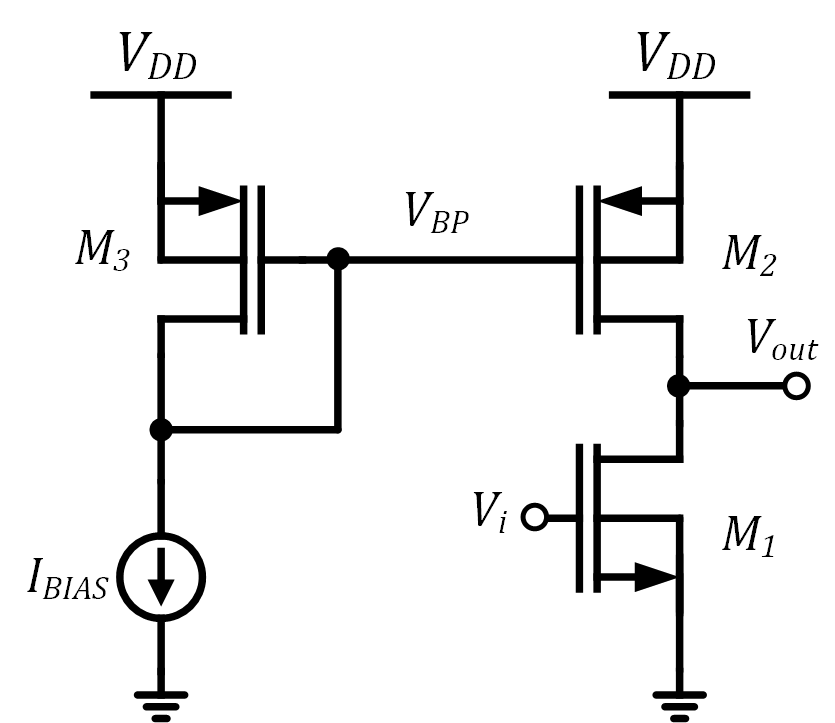
\includegraphics{common_source_biasing.png}
\caption{common\_source\_biasing.png}
\end{figure}

    \begin{figure}
\centering
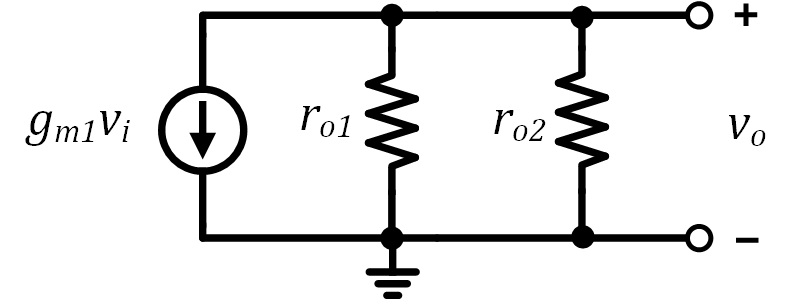
\includegraphics{CS_active_small_signal.png}
\caption{CS\_active\_small\_signal.png}
\end{figure}

\begin{align}
\dfrac{v_o}{v_i} &= -G_m\cdot R_o = g_{m1}\cdot r_{o1} \dfrac{\frac{1}{\lambda_p I_{D2}}}{\frac{1}{\lambda_n I_{D2}} + \frac{1}{\lambda_p I_{D2}}}\\
\\
&= \dfrac{1}{\lambda_n \cdot V_{OV1}}\dfrac{\lambda_n}{\lambda_p + \lambda_n} = \boxed{ \dfrac{g_{m1}r_{o1}}{3} }
\end{align}

    \begin{itemize}
\tightlist
\item
  Compared to the passively-loaded stage, higher gain is achieved by
  increasing output resistance using an active load \(r_{o2}\)
\item
  Bias voltage \(V_{BP}\) is produced using the current mirror formed by
  \(M_2\), \(M_3\)
\end{itemize}

    \hypertarget{current-mirror-sizing}{%
\subsection{Current mirror sizing}\label{current-mirror-sizing}}

    \begin{figure}
\centering
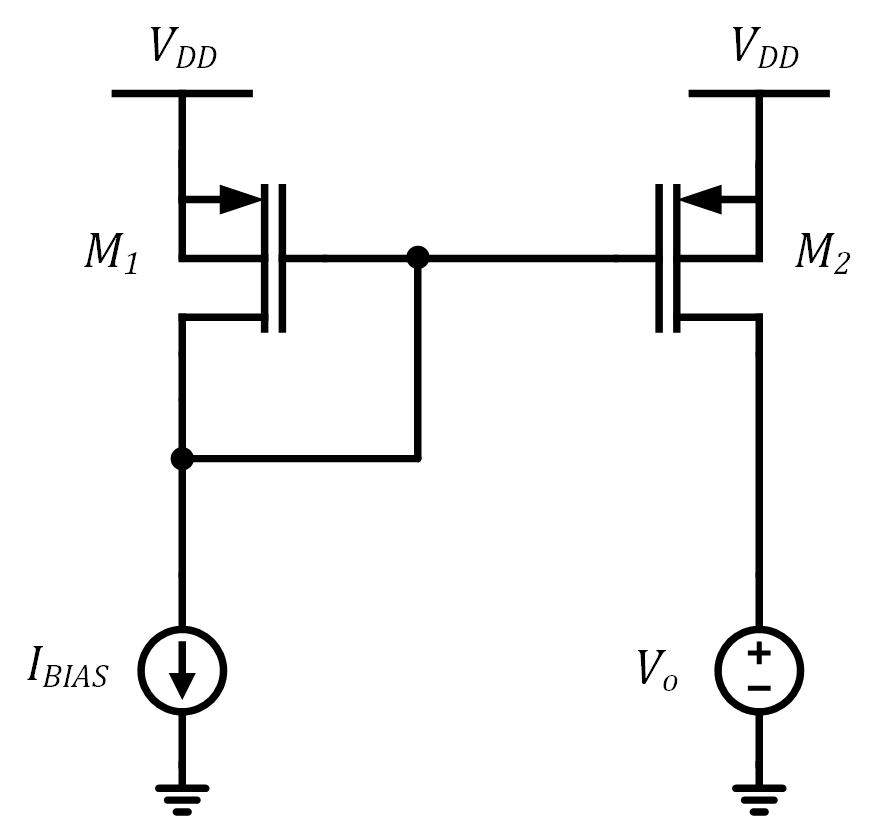
\includegraphics{current_mirror_output_resistance.png}
\caption{current\_mirror\_output\_resistance.png}
\end{figure}

    \begin{equation}
V_{SG2} = V_{SG1}
\end{equation}

\begin{equation}
I_{BIAS} = I_{D1} = \dfrac{1}{2} \mu_p C_{ox}\left(\dfrac{W}{L}\right)_1 (V_{SG1} - |V_{thp}|)^2
\end{equation}

\begin{equation}
I_{D2} =  \dfrac{1}{2} \mu_p C_{ox}\left(\dfrac{W}{L}\right)_2 (V_{SG2} - |V_{thp}|)^2
\end{equation}

\begin{equation}
\dfrac{(W/L)_2}{(W/L)_1} = K \rightarrow \boxed{I_{D2} = K \cdot I_{BIAS}}
\end{equation}

    \begin{itemize}
\tightlist
\item
  When sizing current mirrors, we assume infinite output impedance
  (i.e.~\(\lambda\) = 0) since \(V_o\) isn't constant
\item
  We then select an integer ratio of \((W/L)_2\) to \((W/L)_1\) to
  achieve a specific output current
\end{itemize}

    \hypertarget{current-source-output-resistance}{%
\subsection{Current source output
resistance}\label{current-source-output-resistance}}

    \begin{figure}
\centering
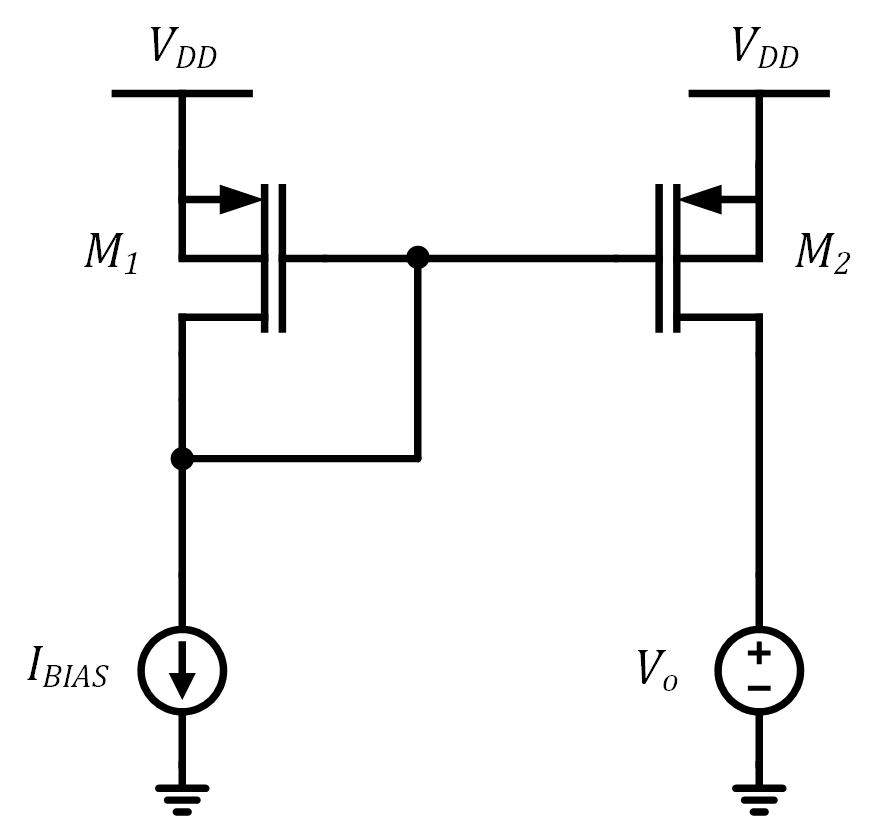
\includegraphics{current_mirror_output_resistance.png}
\caption{current\_mirror\_output\_resistance.png}
\end{figure}

    \begin{align}
\dfrac{1}{R_o} &= \dfrac{\partial I_{D2}}{\partial V_o}\\
\\
&= \dfrac{\partial}{\partial V_o} \dfrac{1}{2} \mu_p C_{ox} \dfrac{W}{L}(V_{SG2} - |V_{thp}|)^2)[1+\lambda_p(V_{DD} - V_o)]\\
\\
&\approx \lambda_p I_{D2} 
\end{align}

\begin{equation}
\rightarrow \boxed{R_o \approx \dfrac{1}{\lambda_p I_{D2}} = r_{o2}} 
\end{equation}

    \begin{itemize}
\tightlist
\item
  The output resistance of a current source determines its sensitivity
  to output voltage
\item
  In the case of a current source based on a single \(MOSFET\), the
  output resistance is equal to the intrinsic output resistance of the
  transistor, \(r_o\)
\end{itemize}

    \begin{itemize}
\tightlist
\item
  Assume that we design our circuit for a nominal operating point of
  \(V_o = 1.5V\) and \(I_{D2} = 100\mu A\)
\end{itemize}

    \begin{tcolorbox}[breakable, size=fbox, boxrule=1pt, pad at break*=1mm,colback=cellbackground, colframe=cellborder]
\prompt{In}{incolor}{16}{\boxspacing}
\begin{Verbatim}[commandchars=\\\{\}]
\PY{n}{lambda\PYZus{}p} \PY{o}{=} \PY{l+m+mf}{0.2}
\PY{n}{V\PYZus{}o} \PY{o}{=} \PY{n}{np}\PY{o}{.}\PY{n}{arange}\PY{p}{(}\PY{l+m+mi}{0}\PY{p}{,} \PY{l+m+mi}{3}\PY{p}{,} \PY{l+m+mf}{0.01}\PY{p}{)}
\PY{n}{I\PYZus{}d2} \PY{o}{=} \PY{n}{pmos\PYZus{}iv\PYZus{}sweep}\PY{p}{(}\PY{l+m+mi}{1}\PY{p}{,} \PY{n}{V\PYZus{}o}\PY{p}{,} \PY{l+m+mi}{100}\PY{p}{,} \PY{l+m+mi}{1}\PY{p}{,} \PY{n}{lambda\PYZus{}p}\PY{p}{)}
\PY{n}{plot\PYZus{}xy}\PY{p}{(}\PY{n}{V\PYZus{}o}\PY{p}{,} \PY{l+m+mf}{1e6}\PY{o}{*}\PY{n}{I\PYZus{}d2}\PY{p}{,} \PY{l+s+sa}{r}\PY{l+s+s1}{\PYZsq{}}\PY{l+s+s1}{\PYZdl{}V\PYZus{}}\PY{l+s+si}{\PYZob{}o\PYZcb{}}\PY{l+s+s1}{\PYZdl{} [V]}\PY{l+s+s1}{\PYZsq{}}\PY{p}{,} \PY{l+s+sa}{r}\PY{l+s+s1}{\PYZsq{}}\PY{l+s+s1}{\PYZdl{}I\PYZus{}}\PY{l+s+si}{\PYZob{}d2\PYZcb{}}\PY{l+s+s1}{\PYZdl{} [\PYZdl{}}\PY{l+s+s1}{\PYZbs{}}\PY{l+s+s1}{mu A\PYZdl{}]}\PY{l+s+s1}{\PYZsq{}}\PY{p}{)}
\end{Verbatim}
\end{tcolorbox}

    \begin{center}
    \adjustimage{max size={0.9\linewidth}{0.9\paperheight}}{2021_01_20_EE538_Lecture3_W2021_files/2021_01_20_EE538_Lecture3_W2021_23_0.png}
    \end{center}
    { \hspace*{\fill} \\}
    
    \begin{itemize}
\tightlist
\item
  The finite output resistance of \(M_2\) causes \(I_{out}\) to vary
  significantly with \(V_o\) (\(\pm20\%\)!)
\item
  This will affect various circuit parameters, such as \(g_m\),
  bandwidth, stability, etc.
\item
  How do we reduce the variability in \(I_{d2}\)?
\end{itemize}

    \hypertarget{source-degeneration}{%
\subsection{Source degeneration}\label{source-degeneration}}

    \begin{figure}
\centering
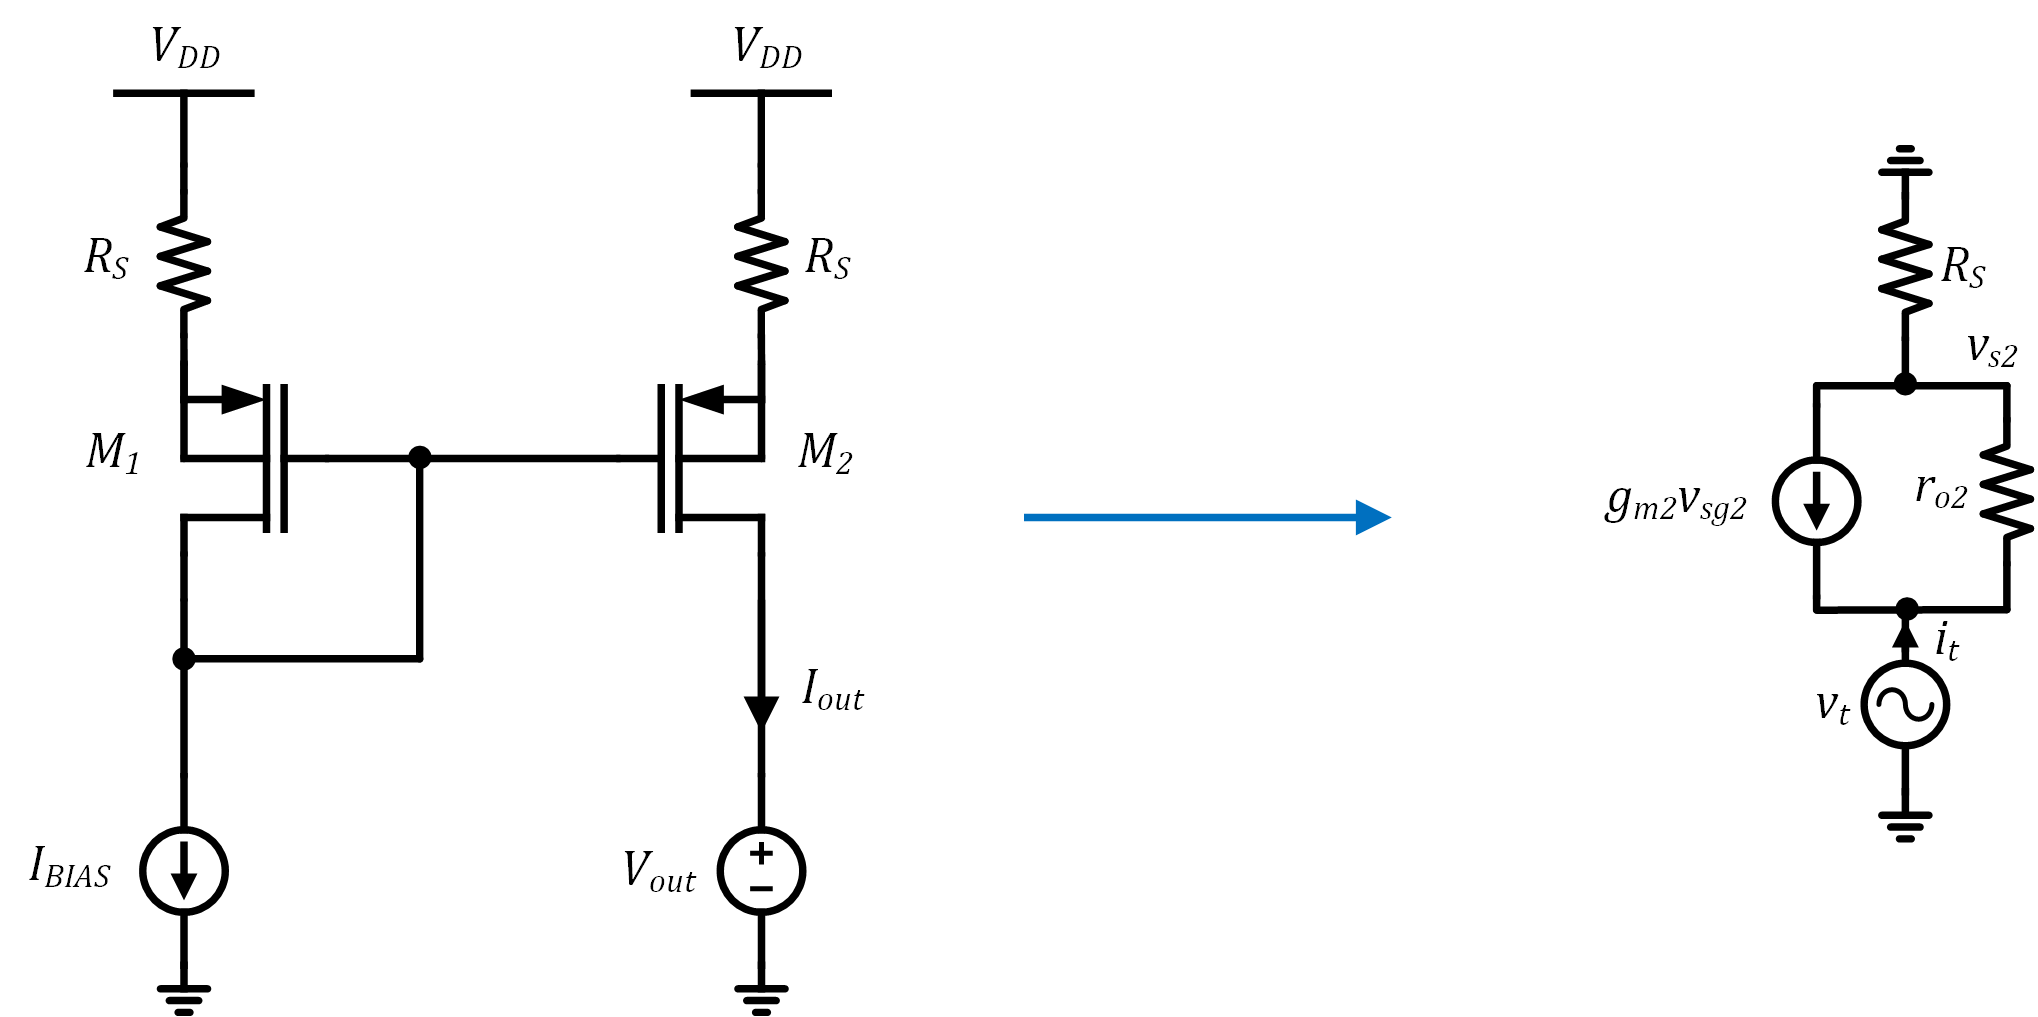
\includegraphics{degenerated_current_mirror.png}
\caption{degenerated\_current\_mirror.png}
\end{figure}

    \begin{equation}
R_o = \dfrac{v_t}{i_t} = ?
\end{equation}

    \begin{itemize}
\tightlist
\item
  Resistor between source of \(PMOS\) and \(V_{DD}\) is referred to as
  ``source degeneration''
\item
  This is a form of negative feedback that increases the output
  resistance of the current source over that of a MOS transistor alone
\end{itemize}

    \hypertarget{small-signal-behavior}{%
\subsection{Small-signal behavior}\label{small-signal-behavior}}

    \begin{figure}
\centering
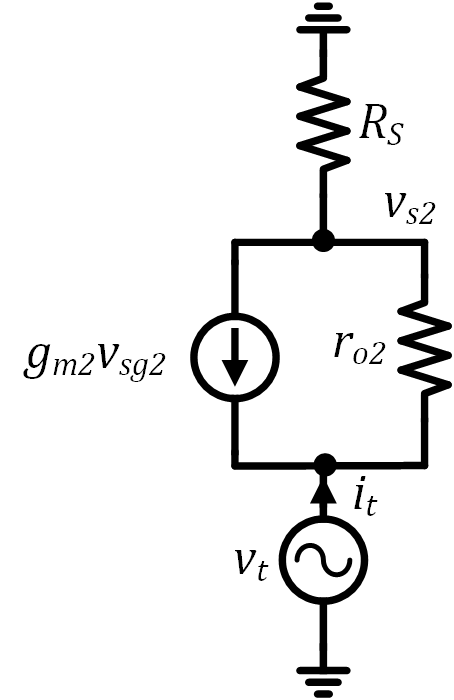
\includegraphics{degeneration_small_signal.png}
\caption{degeneration\_small\_signal.png}
\end{figure}

    \begin{equation}
i_t = \dfrac{v_{s2}}{R_S} = -g_{m2}v_{sg2} + \dfrac{v_t - v_{s2}}{r_{o2}}
\end{equation}

\begin{equation}
v_{s2} = i_t R_S
\end{equation}

\begin{equation}
\boxed{R_o = \dfrac{v_t}{i_t} = r_{o2}(1+g_{m2}R_S) + R_S}
\end{equation}

    \begin{itemize}
\tightlist
\item
  As \(v_t\) increases, so does the source voltage \(v_{s2}\)
\item
  This results in an increase in the current \(g_{m2}v_{s2}\), which is
  in the direction opposite to \(i_t\)
\item
  The resulting negative feedback increases the output resistance of the
  degenerated current source
\end{itemize}

    \hypertarget{increased-output-resistance}{%
\subsection{Increased output
resistance}\label{increased-output-resistance}}

    \begin{itemize}
\tightlist
\item
  If we assume a voltage drop across \(R_S\) of \(200mV\), then
\end{itemize}

\begin{equation}
R_S = \dfrac{0.2V}{I_{D2}}
\end{equation}

\begin{itemize}
\tightlist
\item
  The output resistance of the degenerated current source is
\end{itemize}

\begin{equation}
R_o = r_{o2}(1+g_{m2} R_S) + R_S = r_{o2} \left(1 + \dfrac{2I_{D2}}{V_{OV2}} \dfrac{0.2V}{I_{D2}} \right)+ R_S
\end{equation}

\begin{itemize}
\tightlist
\item
  For \(V_{OV2}\) = \(0.2V\), we obtain
\end{itemize}

\begin{equation}
R_o = 3r_{o2} + R_S \approx 3r_{o2}
\end{equation}

\begin{itemize}
\tightlist
\item
  The original output resistance, \(r_{o2}\), is increased by the gain
  of the feedback loop, \(g_{m2}R_S\), and added to the series
  resistance \(R_S\)
\end{itemize}

    \hypertarget{common-source-amplifier-with-degeneration}{%
\subsection{Common-source amplifier with
degeneration}\label{common-source-amplifier-with-degeneration}}

    \begin{figure}
\centering
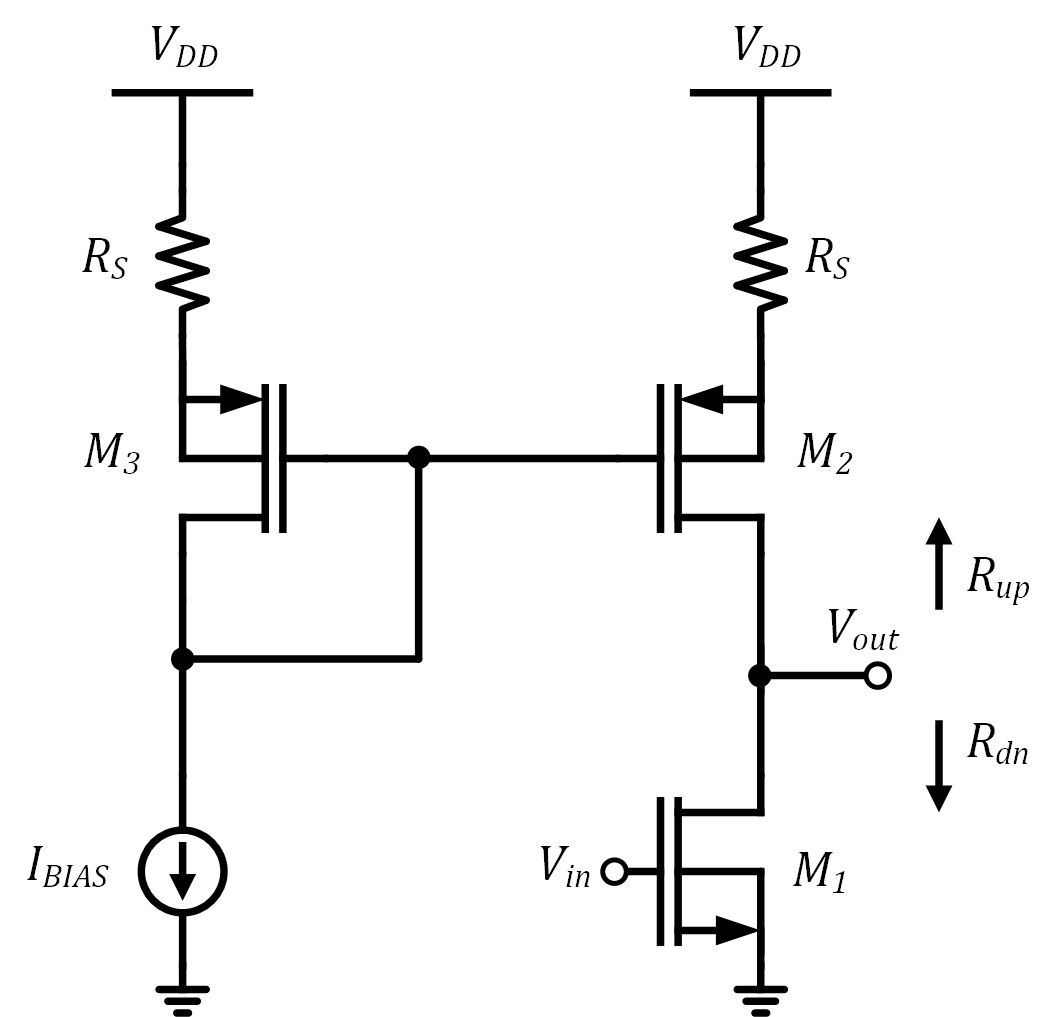
\includegraphics{common_source_degeneration.png}
\caption{common\_source\_degeneration.png}
\end{figure}

    \begin{equation}
R_{up} = r_{o2}(1+g_{m2} R_S) + R_S
\end{equation}

\begin{equation}
R_{dn} = r_{o1}
\end{equation}

\begin{align}
R_o &= R_{up}||R_{dn}\\
\\
&= \left[r_{o2}(1+g_{m2} R_S) + R_S\right] || r_{o1} \\
\end{align}

\begin{equation}
\boxed{ A_v = -g_{m1}R_{o} }
\end{equation}

    \begin{itemize}
\tightlist
\item
  The amplifier output resistance is the parallel combination of the
  current source resistance and \(r_{o1}\)
\item
  Let's take a look at a typical value for this\ldots{}
\end{itemize}

    \begin{itemize}
\tightlist
\item
  Recall that for \(R_S = 0.2V/I_{D2}\) and \(V_{OV2} = 0.2V\), the
  output resistance of the degenerated current source is
\end{itemize}

\begin{equation}
R_{up} = 3r_{o2} + R_S \approx 3r_{o2}
\end{equation}

\begin{itemize}
\tightlist
\item
  This small-signal resistance appears in parallel with
  \(R_{dn} = r_{o1}\), resulting in
\end{itemize}

\begin{equation}
R_o \approx 3r_{o2}||r_{o1}
\end{equation}

\begin{itemize}
\tightlist
\item
  Using our process model parameters \(\lambda_p = 0.2V^{-1}\) and
  \(\lambda_n = 0.1V^{-1}\), we find
\end{itemize}

\begin{equation}
R_o \approx 3r_{o2}||r_{o1} = \dfrac{(\frac{3}{\lambda_p I_{D2}})(\frac{1}{\lambda_n I_{D2}})}{\frac{3}{\lambda_p I_{D2}} + \frac{1}{\lambda_n I_{D2}}} = \dfrac{(\frac{3}{\lambda_p I_{D2}})(\frac{1}{\lambda_n I_{D2}})}{\frac{3\lambda_n + \lambda_p}{\lambda_n \lambda_p I_{D2}}} = \dfrac{3}{(3\lambda_n + 2\lambda_n)I_{D2}} = \dfrac{3}{5}r_{on}
\end{equation}

\begin{itemize}
\tightlist
\item
  We have increased the output resistance (and hence the gain) of the
  common-source amplifier by about 20\%
\item
  Can we do better?
\end{itemize}

    \begin{itemize}
\tightlist
\item
  What if \(R_S = r_{op}\)?
\item
  In this case, the output resistance of the current source becomes
\end{itemize}

\begin{equation}
R_{up} = r_{op}(1+g_{m2} r_{op}) + r_{op}
\end{equation}

\begin{itemize}
\tightlist
\item
  \(g_{m2} r_{op}\) is equal to the intrinsic gain of a \(PMOS\)
  transistor. If we take this to be at least \(10V/V\), the current
  source output impedance becomes
\end{itemize}

\begin{equation}
R_{up} = r_{op}(1+g_{m2} r_{op}) + r_{op} \geq 12 r_{op}
\end{equation}

\begin{itemize}
\tightlist
\item
  This is more than an order of magnitude higher than the output
  impedance of a single transistor. How do we achieve this?
\end{itemize}

    \hypertarget{common-source-amplifier-with-cascode-load}{%
\subsection{Common-source amplifier with cascode
load}\label{common-source-amplifier-with-cascode-load}}

    \begin{figure}
\centering
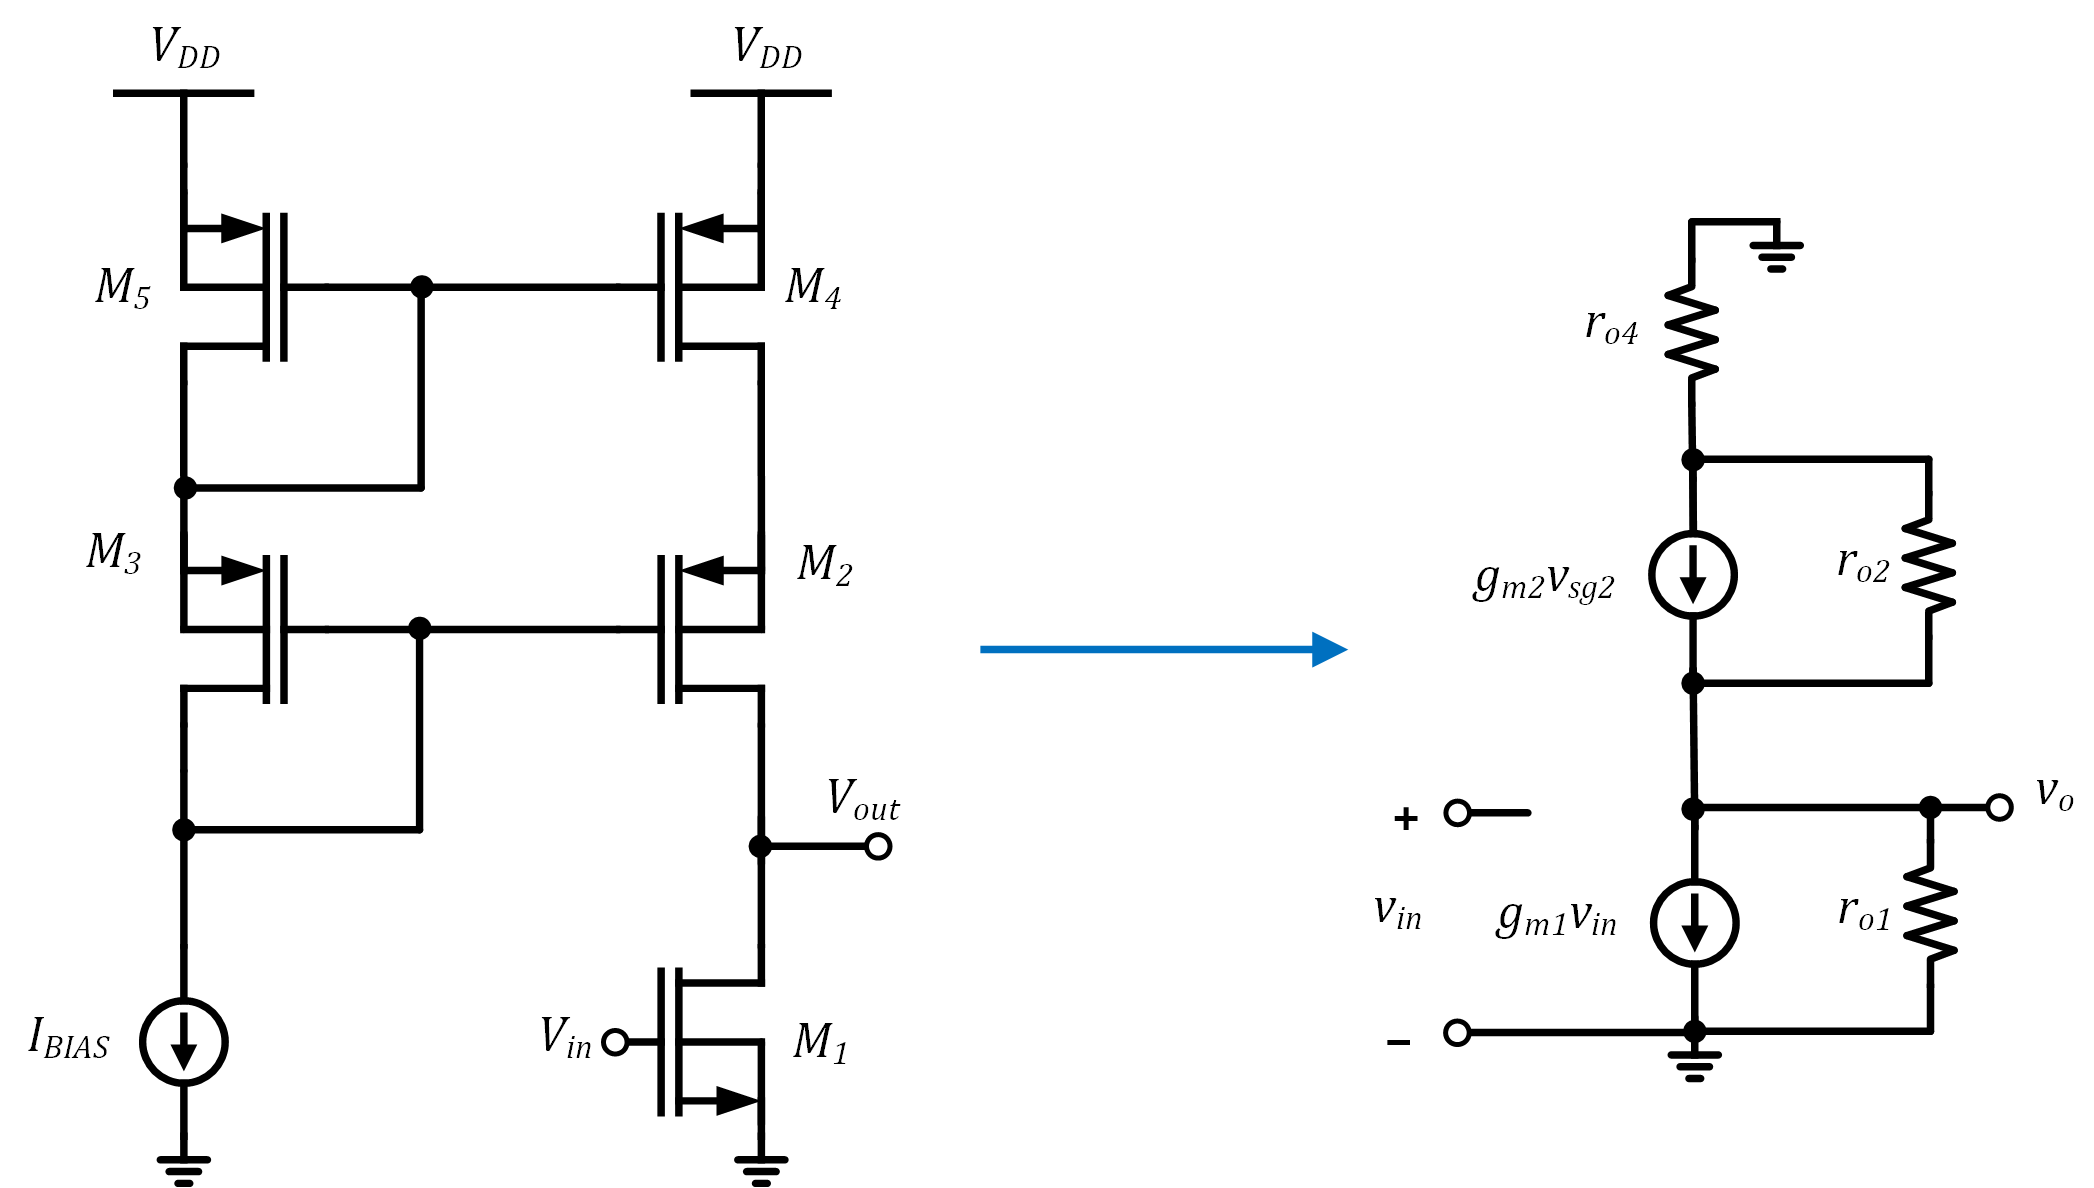
\includegraphics{common_source_cascode_load.png}
\caption{common\_source\_cascode\_load.png}
\end{figure}

    \begin{itemize}
\tightlist
\item
  ``Cascoding'' is source degeneration using \(r_o\) in place of \(R_S\)
\item
  The \(DC\) gain of this configuration is
\end{itemize}

\begin{equation}
A_v = -G_m \cdot R_o = -g_{m1}\cdot r_{o1}||\left[r_{o2}(1+g_{m2} r_{o4}) + r_{o4}\right] \approx -g_{m1}r_{o1}
\end{equation}

\begin{itemize}
\tightlist
\item
  By setting the output impedance of the current source to be much
  greater than that of \(M_1\), our gain is nearly equal to the
  intrinsic gain of \(M_1\)
\end{itemize}

    \hypertarget{summary-so-far}{%
\subsection{Summary (so far)}\label{summary-so-far}}

    \begin{itemize}
\tightlist
\item
  Common-source amplifier with resistive load provides only modest gain
\end{itemize}

\begin{equation}
|A_v| \approx g_{m1}R_D = \dfrac{2I_{D1}}{V_{OV1}}\dfrac{V_{DD}/2}{I_{D1}} = \dfrac{V_{DD}}{V_{OV1}}
\end{equation}

\begin{itemize}
\tightlist
\item
  An active load increases this slightly
\end{itemize}

\begin{equation}
|A_v| = g_{m1} \cdot r_{o1}||r_{o2} \approx g_{m1}\dfrac{r_{o1}}{3}
\end{equation}

\begin{itemize}
\tightlist
\item
  Source degeneration increases output resistance of current source and
  (slightly) increases gain
\end{itemize}

\begin{equation}
|A_v| = g_{m1}\cdot r_{o1}||\left[r_{o2}(1+g_{m2} R_{S}) + R_{S}\right] \approx \dfrac{3}{5}g_{m1}r_{o1}
\end{equation}

\begin{itemize}
\tightlist
\item
  The cascode current source significantly increases output resistance
  of the current source/active load
\end{itemize}

\begin{equation}
|A_v| = g_{m1}\cdot r_{o1}||\left[r_{o2}(1+g_{m2} r_{o4}) + r_{o4}\right] \approx g_{m1}r_{o1}
\end{equation}

    \hypertarget{common-source-with-cascode-load}{%
\subsection{Common-source with cascode
load}\label{common-source-with-cascode-load}}

    \begin{figure}
\centering
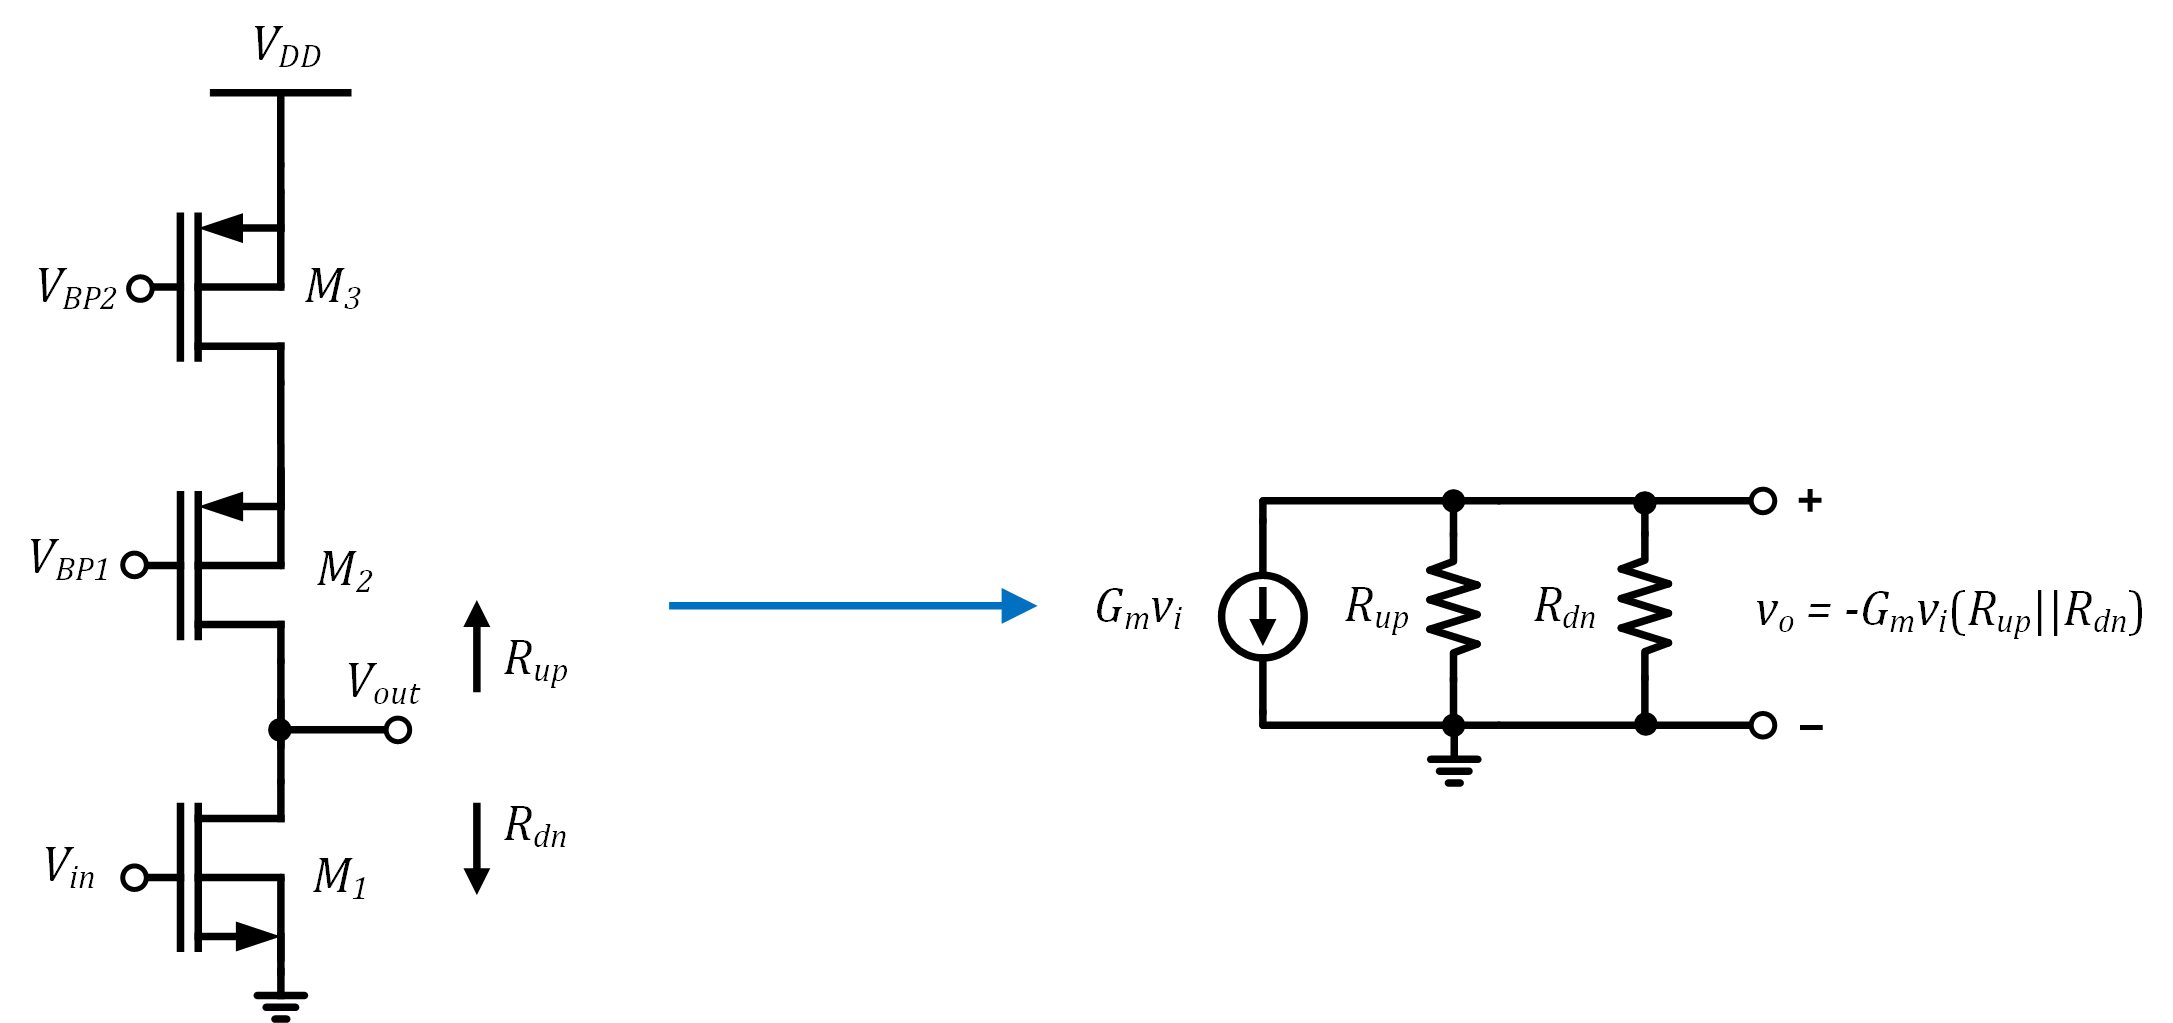
\includegraphics{CS_cascode_load_model.png}
\caption{CS\_cascode\_load\_model.png}
\end{figure}

    \begin{itemize}
\tightlist
\item
  \(R_{up} \approx g_{m2}r_{o2}r_{o3}\), while \(R_{dn} = r_{o1}\)
\item
  Cascode current-source load impedance (\(R_{up}\)) is
  \textasciitilde{}\(g_m r_o\) times higher than \(r_{o1}\) (\(R_{dn}\))
\item
  If we can increase \(R_{dn}\) by the same factor, we can significantly
  increase our gain
\item
  How do we accomplish this?
\end{itemize}

    \hypertarget{cascode-amplifier}{%
\subsection{Cascode amplifier}\label{cascode-amplifier}}

    \begin{figure}
\centering
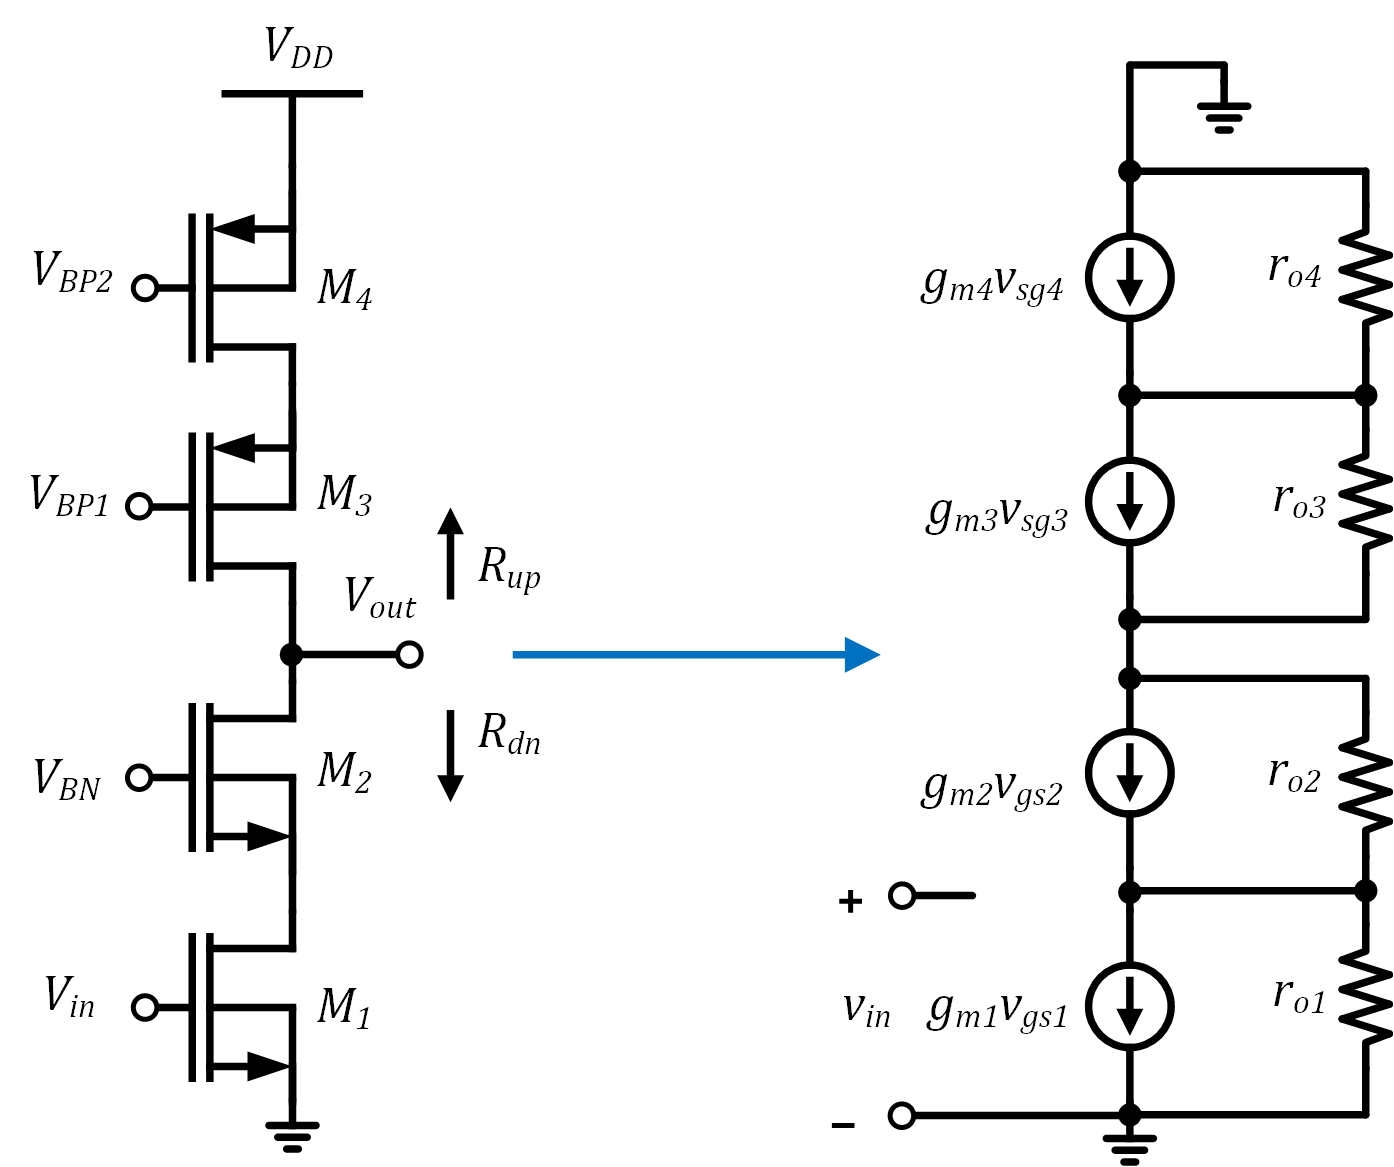
\includegraphics{cascode_amplifier.png}
\caption{cascode\_amplifier.png}
\end{figure}

    \begin{itemize}
\tightlist
\item
  A ``fully cascoded'' amplifier consists of symmetric stacks of
  \(NMOS\) and \(PMOS\) devices
\item
  Recall that \(R_{up}\) is given by
\end{itemize}

\begin{equation}
R_{up} = r_{o3}(1+g_{m3} r_{o4}) + r_{o4} \approx g_{m3}r_{o3}r_{o4}
\end{equation}

\begin{itemize}
\tightlist
\item
  What about \(R_{dn}\)?
\end{itemize}

    \hypertarget{cascode-amplifier-output-impedance-ro}{%
\subsection{Cascode amplifier output impedance
(Ro)}\label{cascode-amplifier-output-impedance-ro}}

    \begin{figure}
\centering
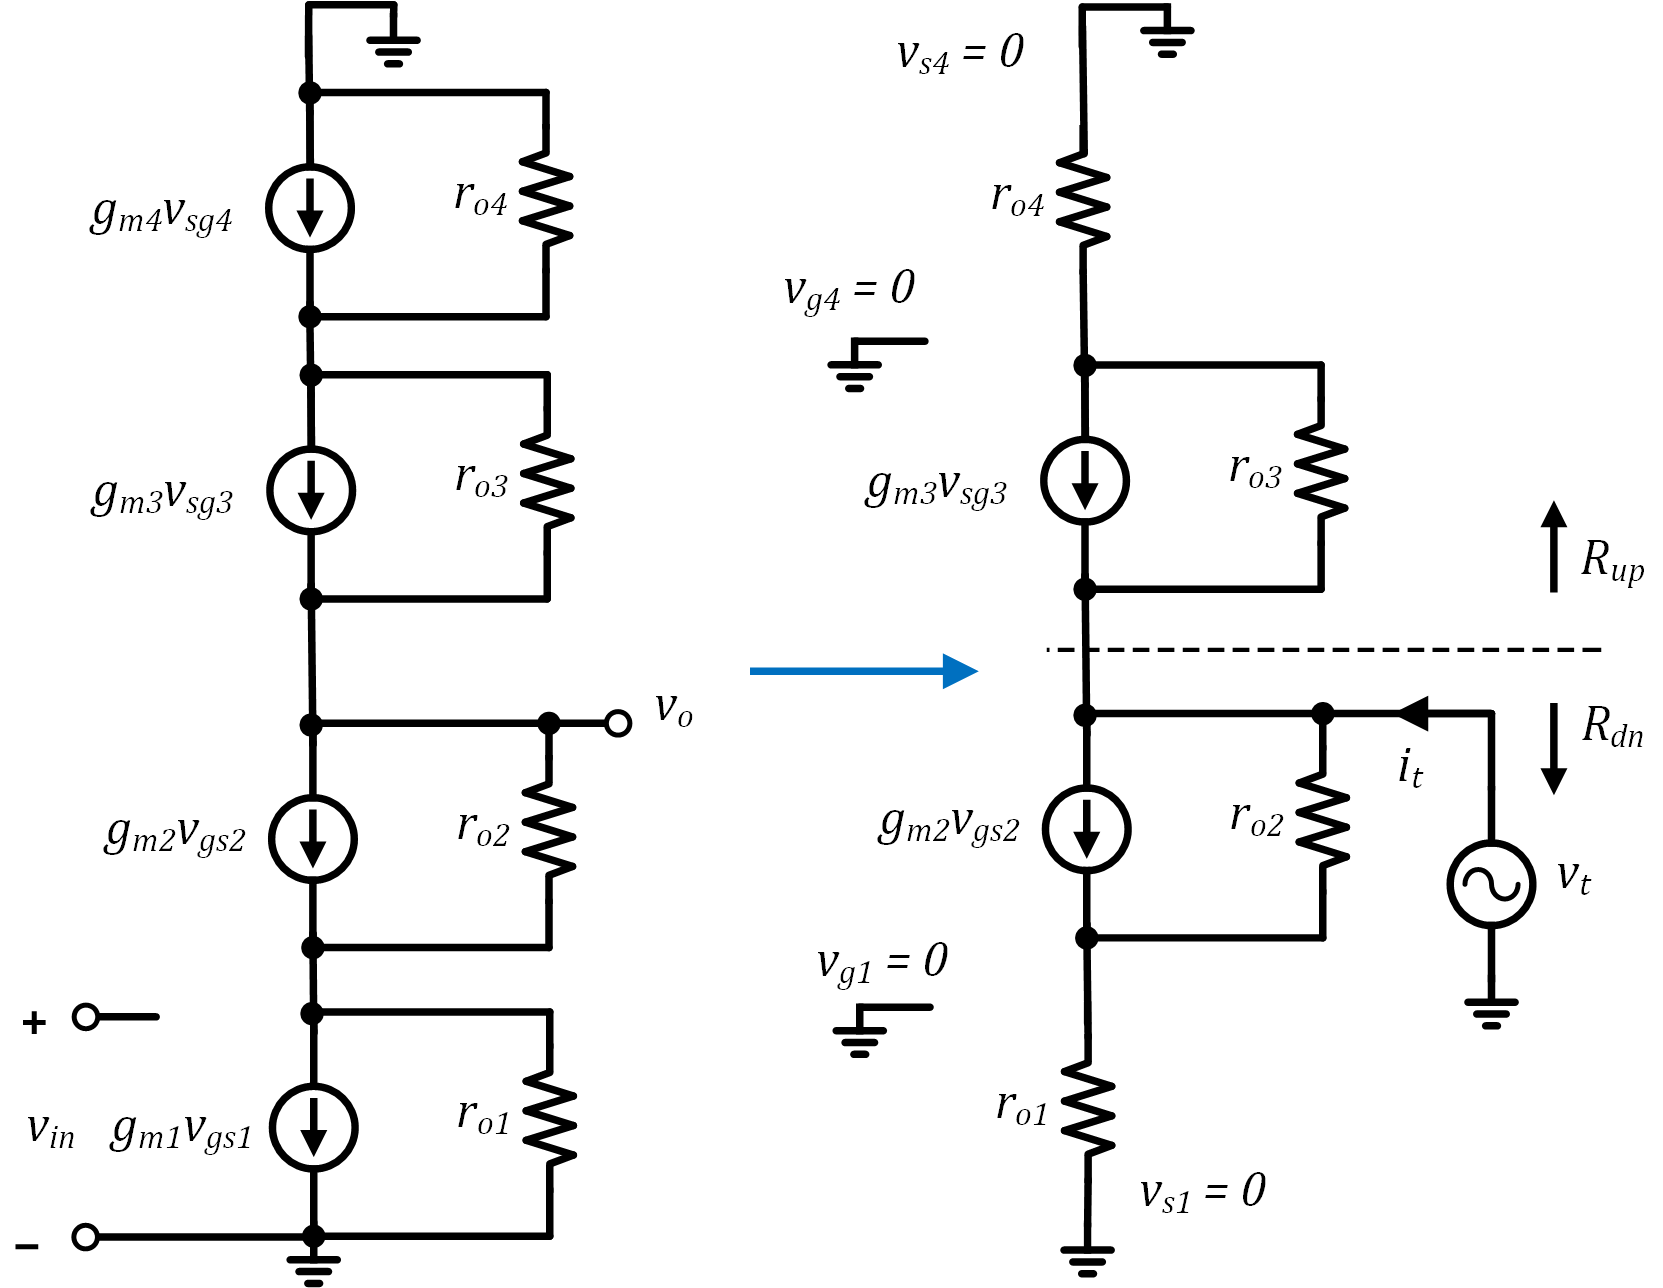
\includegraphics{cascode_amplifier_Ro.png}
\caption{cascode\_amplifier\_Ro.png}
\end{figure}

    \begin{itemize}
\tightlist
\item
  Input voltage (\(v_{g1}\)) is set to zero when determining \(R_o\)
  (Thevenin approach)
\item
  Based on the symmetry of \(R_{up}\), \(R_{dn}\), we can directly write
\end{itemize}

\begin{equation}
R_{up} = r_{o2}(1+g_{m2} r_{o1}) + r_{o1} \approx g_{m2}r_{o2}r_{o1}
\end{equation}

\begin{itemize}
\tightlist
\item
  The output impedance is the parallel combination of the two:
\end{itemize}

\begin{equation}
R_{up} \approx g_{m2}r_{o2}r_{o1}||g_{m3}r_{o3}r_{o4}
\end{equation}

    \hypertarget{cascode-amplifier-output-impedance-gm}{%
\subsection{Cascode amplifier output impedance
(Gm)}\label{cascode-amplifier-output-impedance-gm}}

    \begin{figure}
\centering
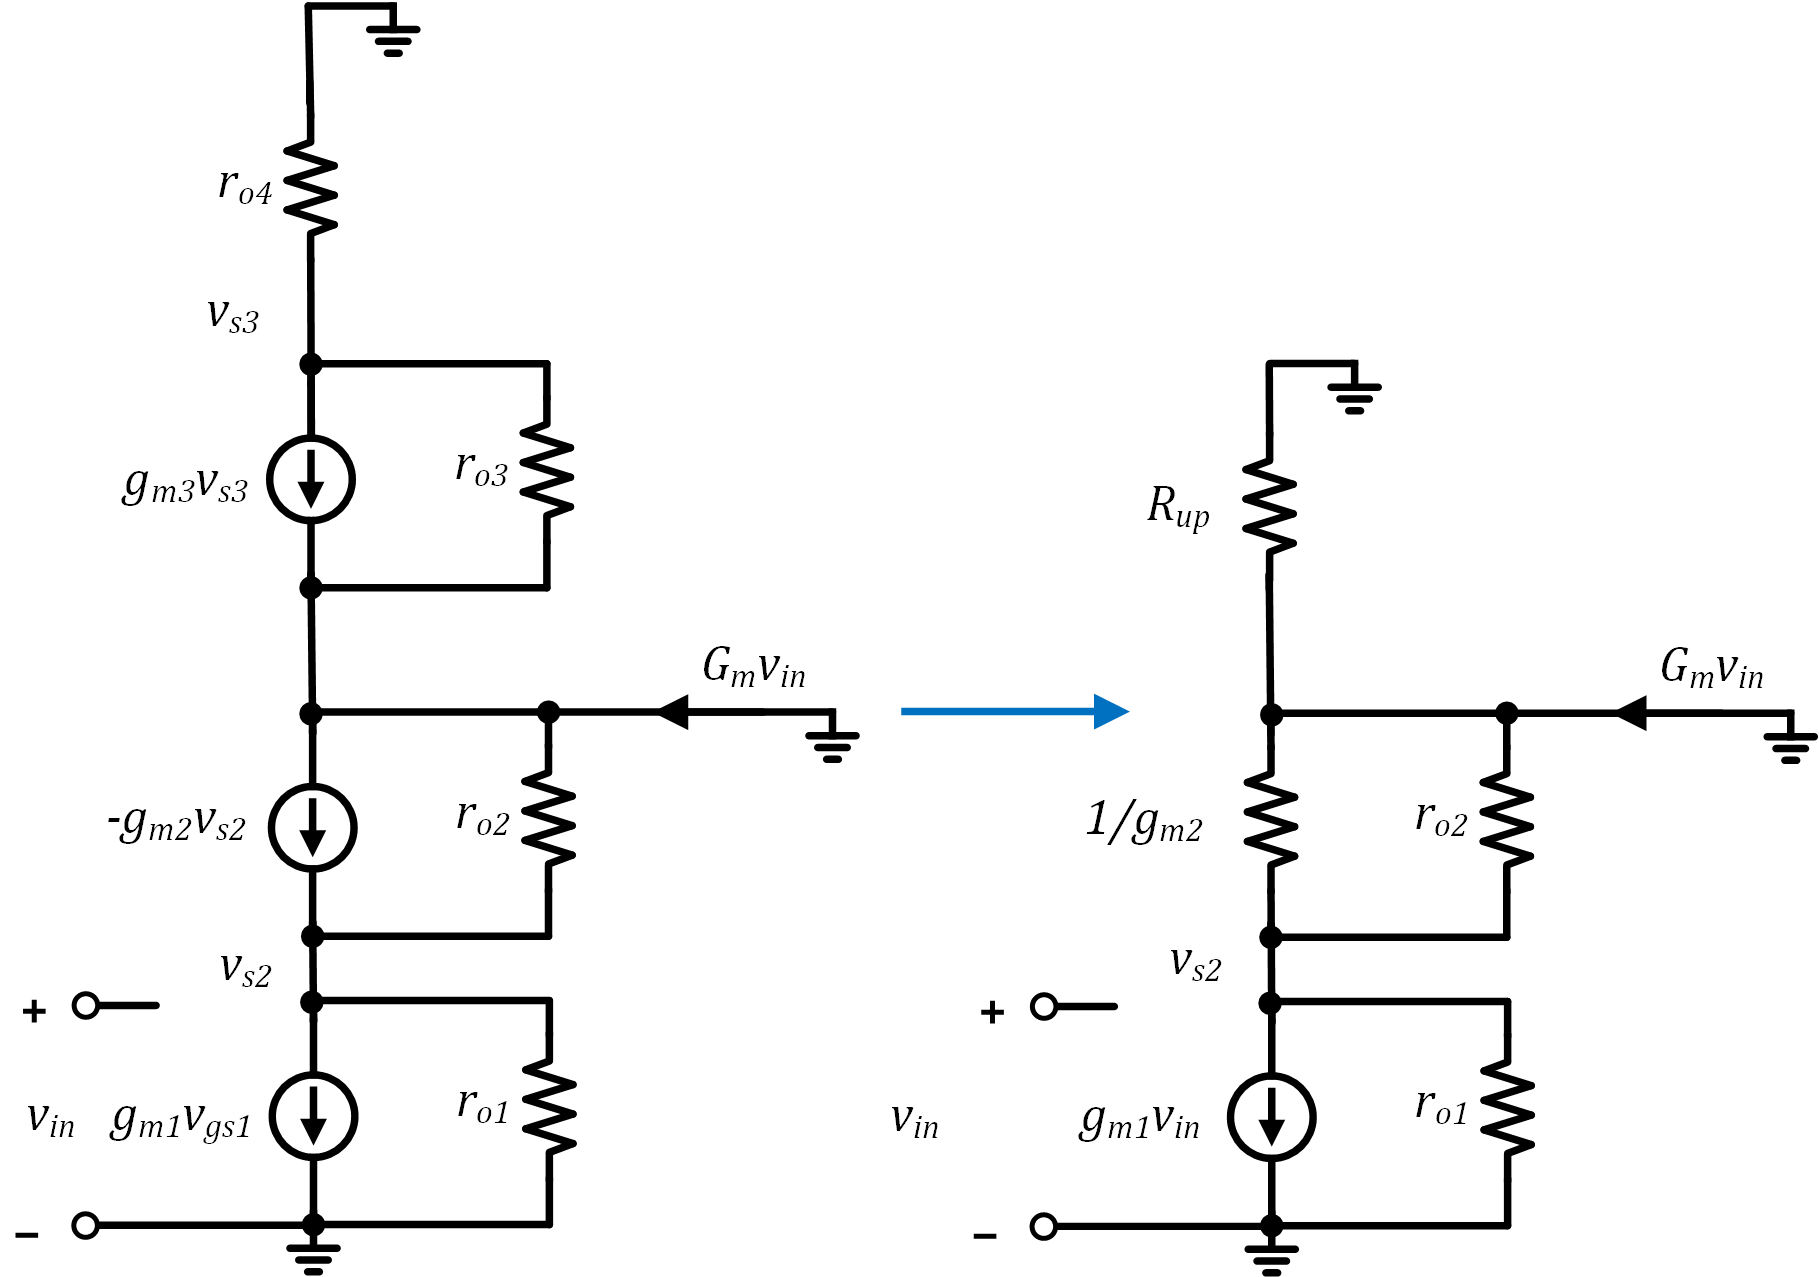
\includegraphics{cascode_amplifier_Gm.png}
\caption{cascode\_amplifier\_Gm.png}
\end{figure}

    \begin{itemize}
\tightlist
\item
  Current through \(r_{o1}\) shunted by parallel combination of
  \(1/g_{m2}\) and \(r_{o2}\):
\end{itemize}

\begin{equation}
G_m v_{in} = g_{m1}v_{in}\cdot\dfrac{r_{o1}}{\frac{1}{g_{m2}}||r_{o2} + r_{o1}} \approx g_{m1}v_{in}
\end{equation} - As long as \(r_{o1},r_{o2} >> 1/g_{m1}\), \(G_m\) is
approximately equal to \(g_{m1}\)

    \hypertarget{cascode-amplifier-voltage-gain}{%
\subsection{Cascode amplifier voltage
gain}\label{cascode-amplifier-voltage-gain}}

    \begin{figure}
\centering
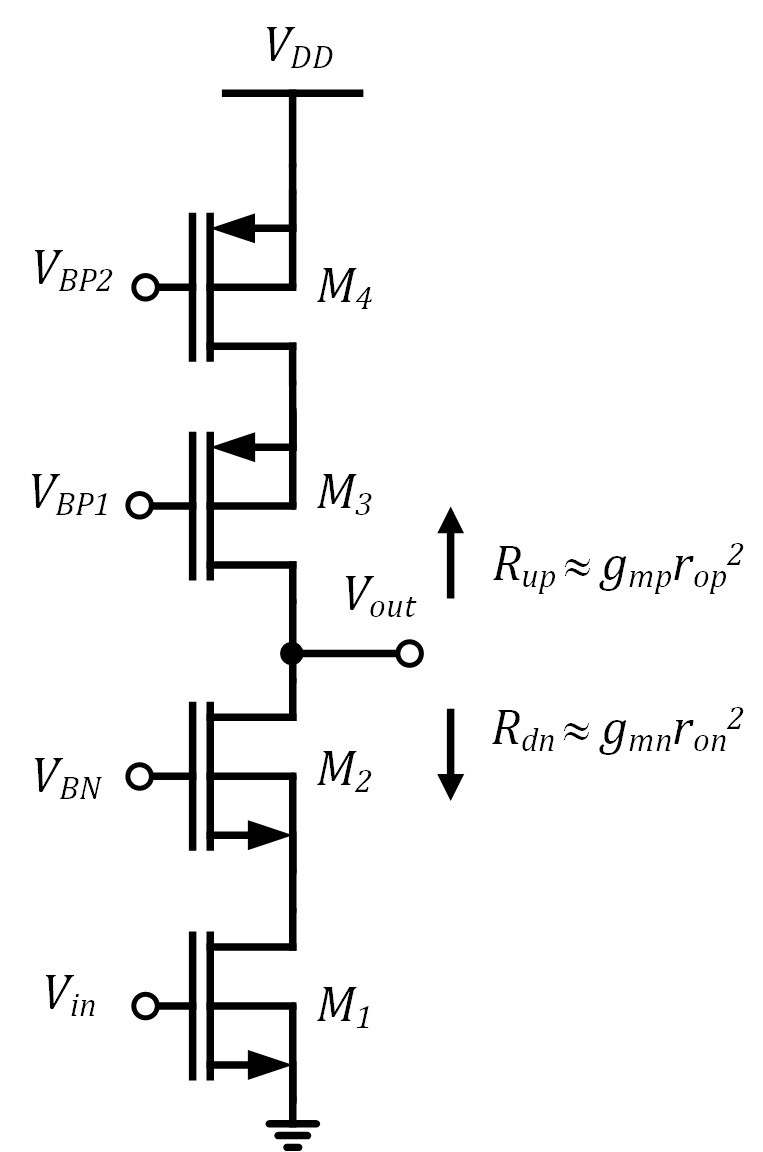
\includegraphics{cascode_simple_Ro.png}
\caption{cascode\_simple\_Ro.png}
\end{figure}

    \begin{align}
A_v &= \dfrac{v_{out}}{v_{in}} \\
\\
&= -G_m\cdot R_o \\
\\
&\approx \boxed{-g_{m1}[g_{m3}r_{op}^2||g_{m2}r_{on}^2]}
\end{align}

    \begin{itemize}
\tightlist
\item
  \(R_{up}\) and \(R_{dn}\) both based on \(r_o\) and scaled by
  \(g_mr_o\) (degeneration)
\item
  Gain is approximately \(g_mr_o\) times higer than that of a common
  source with active load
\item
  Let's put some numbers to this\ldots{}
\end{itemize}

    \begin{itemize}
\tightlist
\item
  In our Level 1 model, \(\lambda_n = 0.1V^{-1}\)
\item
  To achieve high gain, we want to use a relatively low overdrive
  voltage, say \(200mV\)
\item
  For simplicity, let's assume \(g_{mn}r_{on} = g_{mp}r_{op} = g_mr_o\).
  The cascode amplifier gain is thus
\end{itemize}

\begin{equation}
|A_v| \approx \dfrac{g_m^2r_o^2}{2} = \left( \dfrac{I_D}{V_{OV}}\dfrac{1}{\lambda I_D} \right)^2 = 2,500 V/V
\end{equation}

\begin{itemize}
\tightlist
\item
  By ``cascoding,'' we increase our gain from \(30dB\) with a resistive
  load to nearly \(70dB\)!
\item
  Our actual gain will typically be a bit lower than this, since \(g_m\)
  and \(r_o\) won't be the same for all devices
\end{itemize}

    \hypertarget{cascode-bulk-connections}{%
\subsection{Cascode bulk connections}\label{cascode-bulk-connections}}

    \begin{figure}
\centering
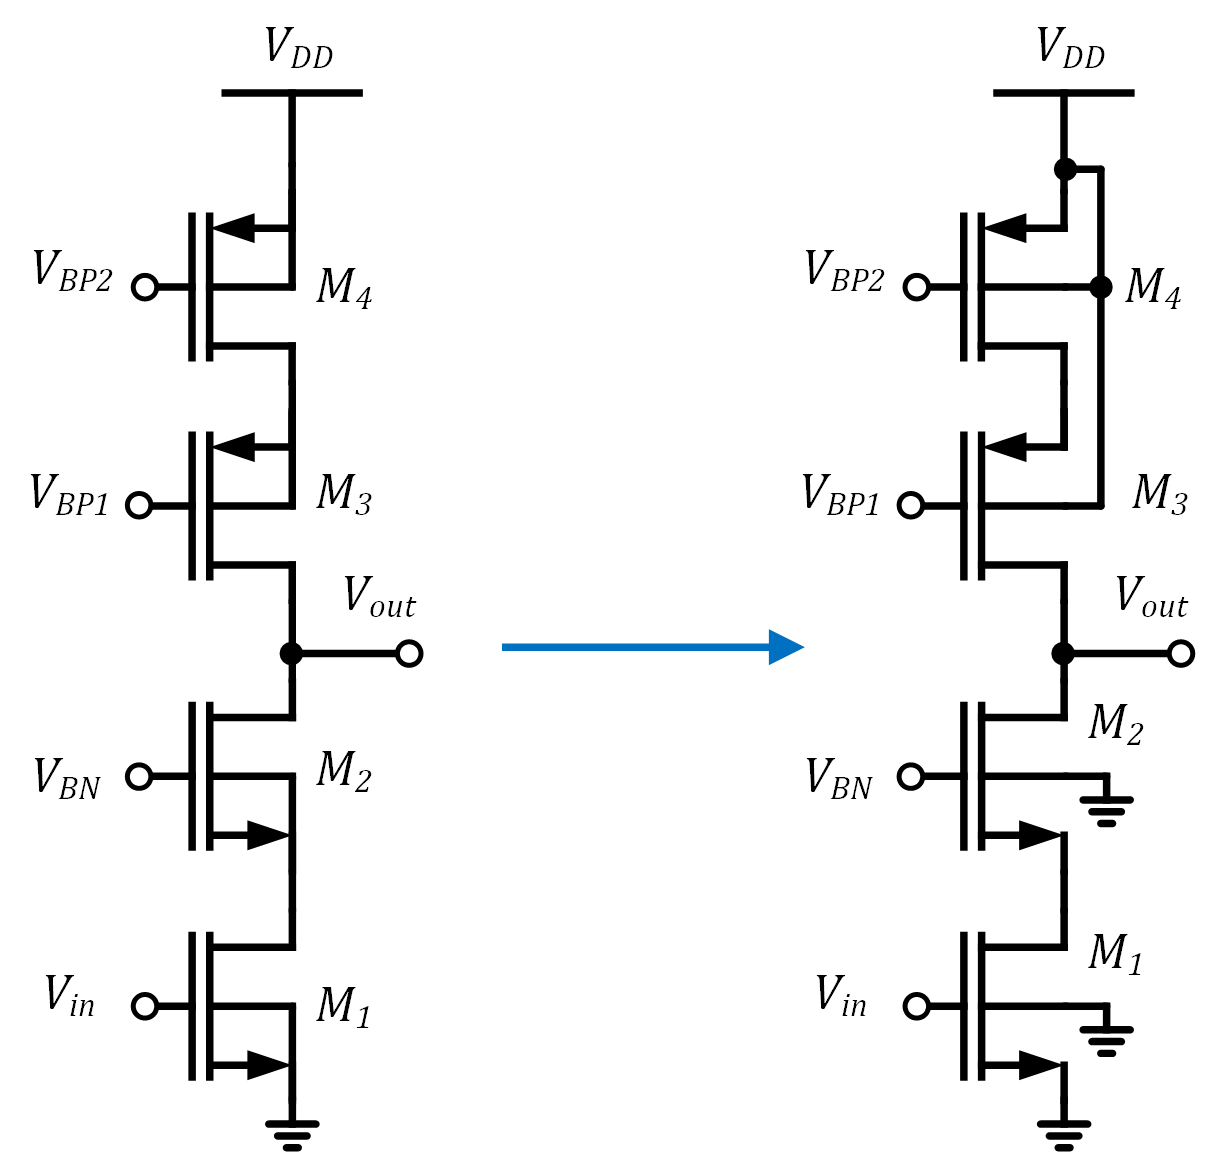
\includegraphics{cascode_bulk_connections.png}
\caption{cascode\_bulk\_connections.png}
\end{figure}

    \begin{itemize}
\tightlist
\item
  In the cascode and source-dengerated structures, \(PMOS\)/\(NMOS\)
  source terminals may not be connected to \(V_{DD}\)/\(GND\)
\item
  Whereas \(PMOS\) devices are fabricated in \emph{n-wells} and can have
  independent source potentials, \(NMOS\) bulks comprise the chip
  substrate and must be biased at the same potential (\(0V\), in most
  cases)
\item
  Both the large- and small-signal behavior of the \(MOSFET\) are
  affected by nonzero values of \(V_{bs}\) via modulation of the
  threshold voltage
\end{itemize}

    \hypertarget{definition-of-threshold-voltage}{%
\subsection{Definition of threshold
voltage}\label{definition-of-threshold-voltage}}

    \begin{figure}
\centering
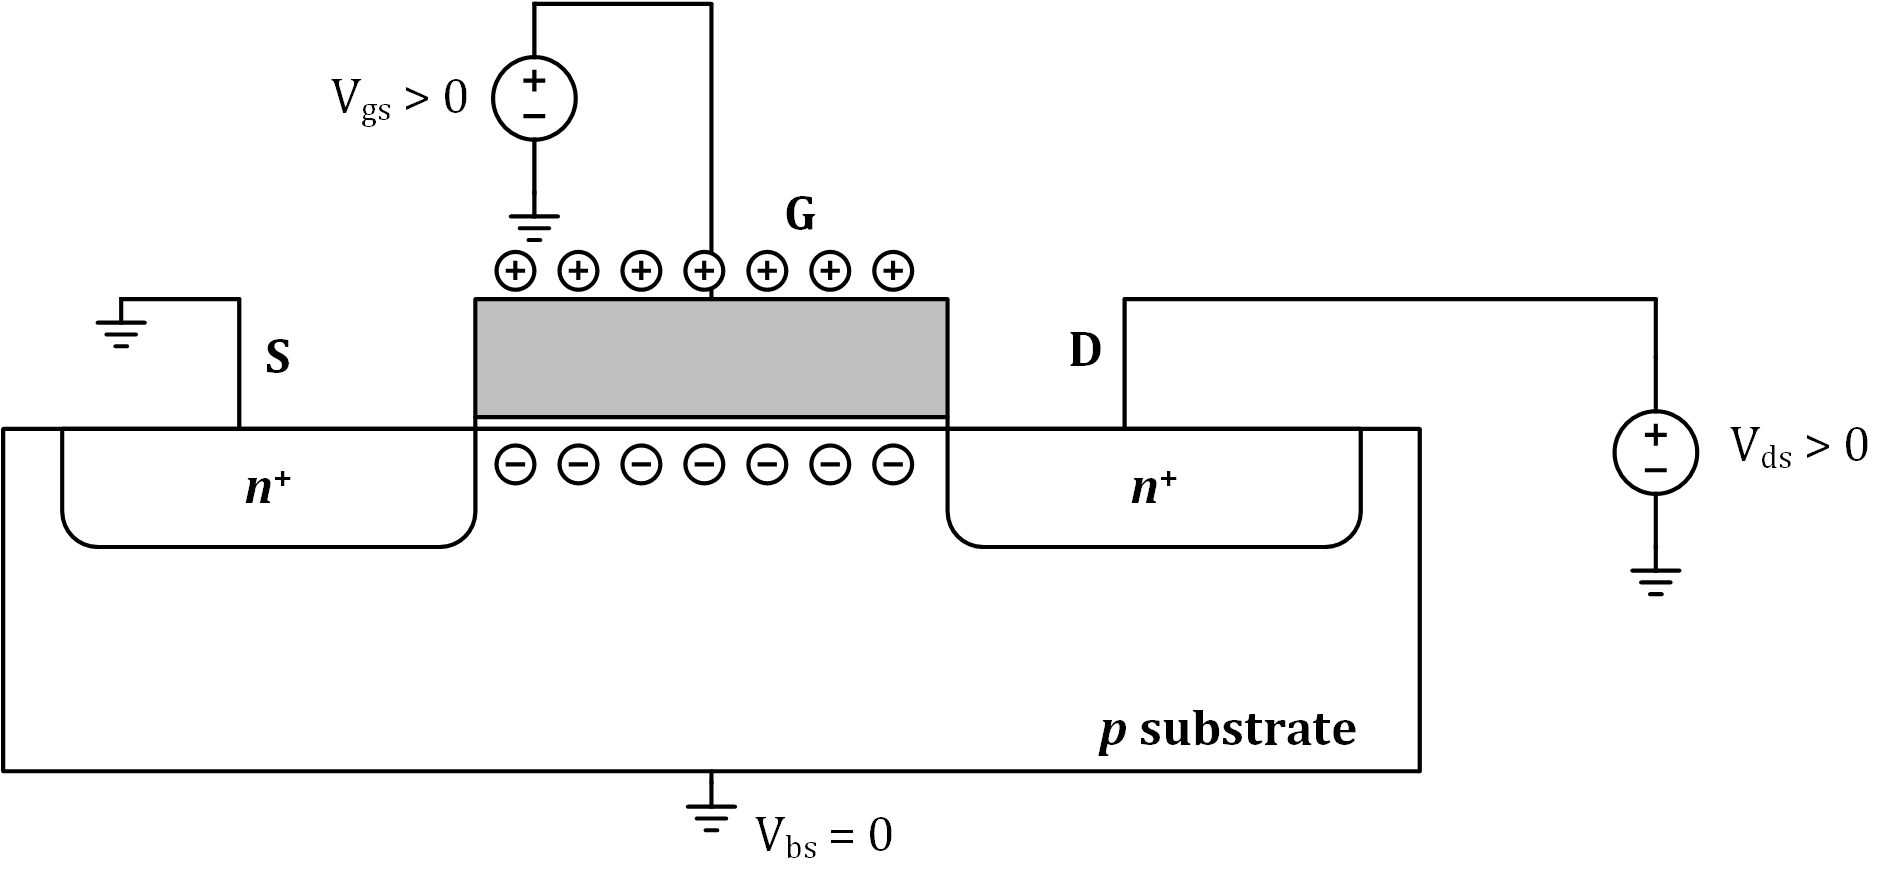
\includegraphics{NMOS_threshold_voltage.png}
\caption{NMOS\_threshold\_voltage.png}
\end{figure}

    \begin{itemize}
\tightlist
\item
  As \(V_{gs}\) increases from \(0\), holes are repelled from the
  substrate region under the gate, leaving behind a negatively-charged
  depletion region
\item
  Charge balance requries that positive gate charge mirror the immobile
  depletion charge
\item
  As \(V_{gs}\) continues to increase, electrons are attracted from
  source and drain to form an inversion layer
\end{itemize}

    \hypertarget{body-effect-vbs-0}{%
\subsection{Body effect (Vbs \textless{} 0)}\label{body-effect-vbs-0}}

    \begin{figure}
\centering
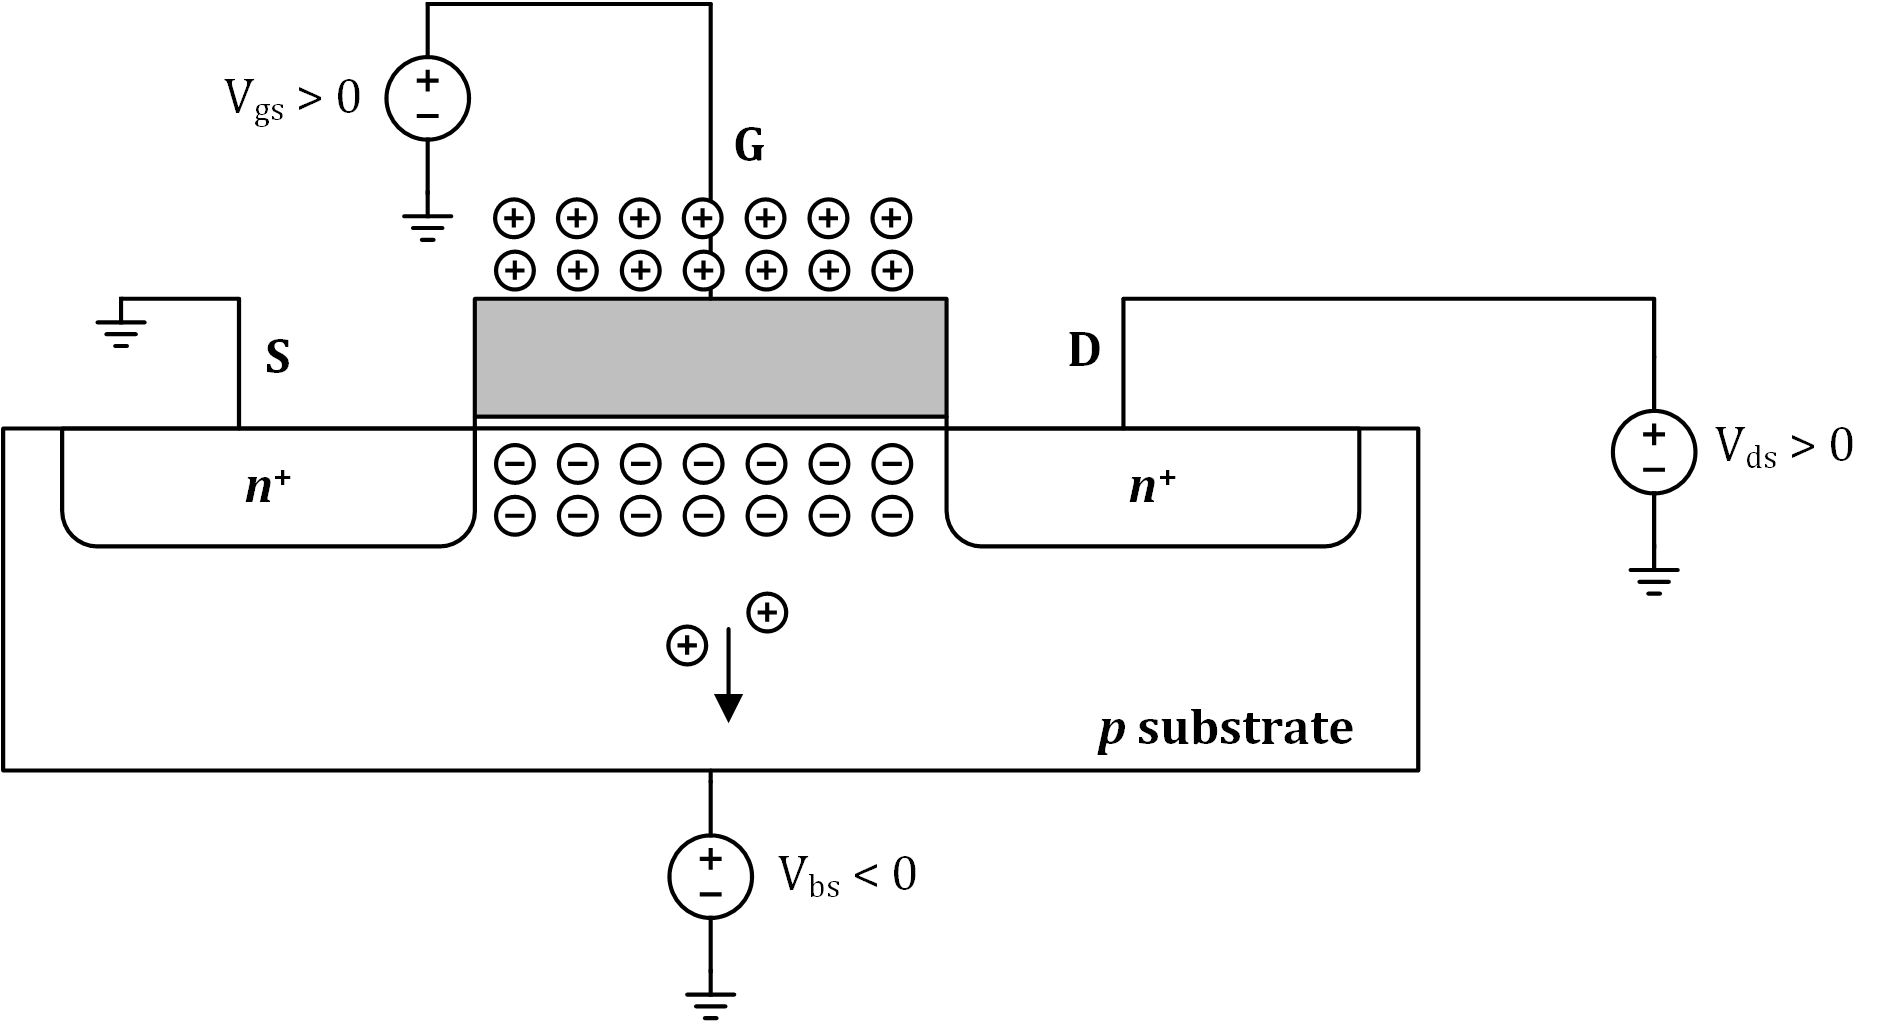
\includegraphics{NMOS_body_effect.png}
\caption{NMOS\_body\_effect.png}
\end{figure}

    \begin{itemize}
\tightlist
\item
  For \(V_{bs} < 0\), some holes are pulled from the interface toward
  the bulk terminal, resulting in more negative charge in the depletion
  region
\item
  More positive gate charge is thus required to form an inversion layer,
  increasing \(V_{th}\)
\item
  The threshold voltage thus increases with increasing \(V_{sb}\), and
  is defined as
\end{itemize}

\begin{equation}
V_{th} = V_{th0} + \gamma (\sqrt{2\phi_F + V_{sb}} - \sqrt{2\phi_F})
\end{equation}

    \hypertarget{body-effect-small-signal}{%
\subsection{Body effect (small signal)}\label{body-effect-small-signal}}

    \begin{figure}
\centering
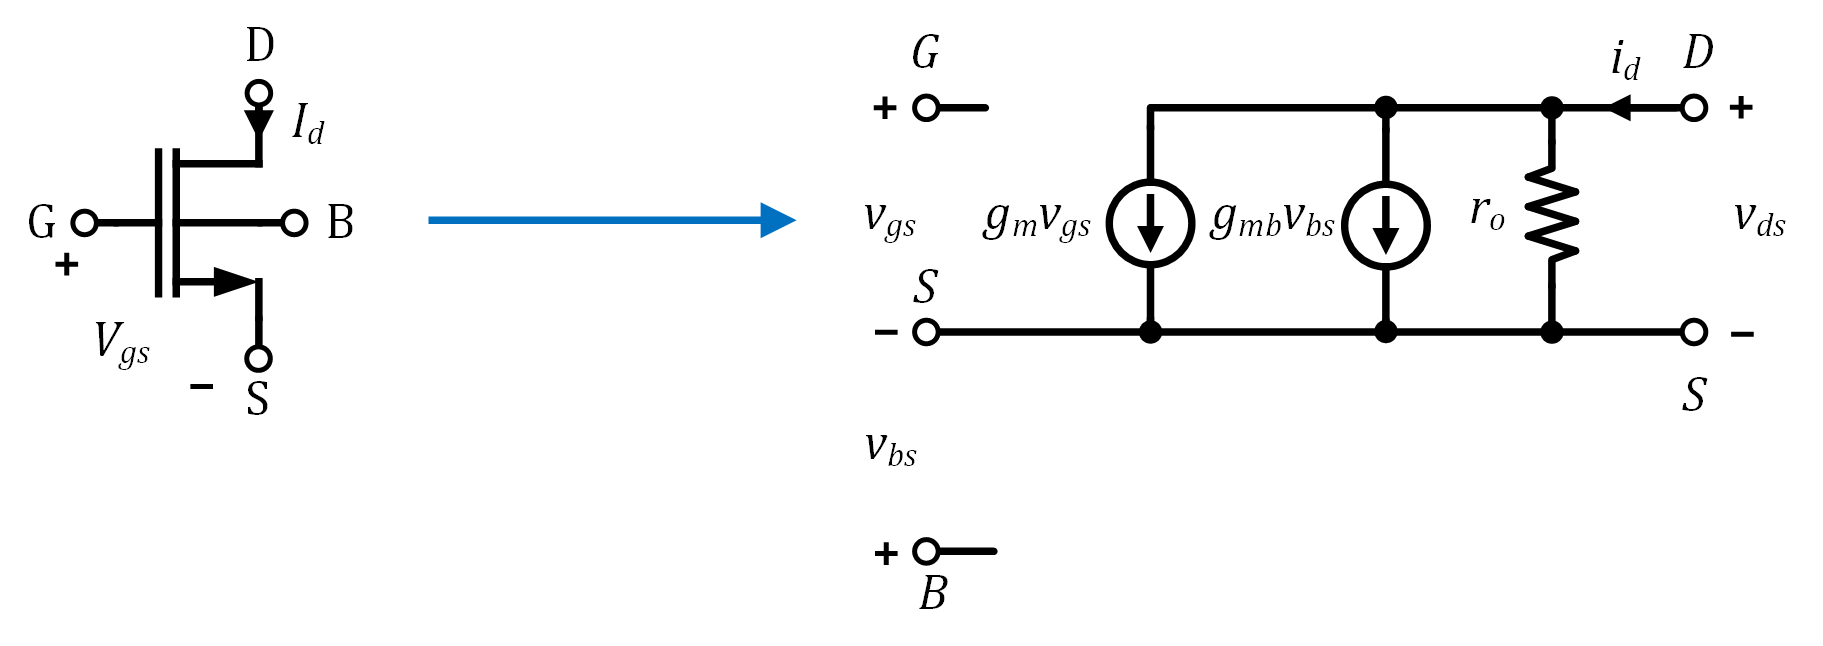
\includegraphics{body_effect_small_signal.png}
\caption{body\_effect\_small\_signal.png}
\end{figure}

    \begin{equation}
g_{mb} = \dfrac{\partial I_D}{\partial V_{BS}} = g_m \dfrac{\gamma}{2\sqrt{2\phi_F + V_{SB}}} = \eta g_m
\end{equation}

    \begin{itemize}
\tightlist
\item
  When \(v_{bs} \neq 0\), the bulk terminal acts as a second ``gate''
  (body effect is often referred to as the ``back-gate'' effect)
\item
  A typical range for \(\gamma\) is between \(0.1\) and \(0.5\),
  depending on the process technology
\item
  Affects source-degenerated, cascode, source follower, and common-gate
  configurations
\item
  Only needs to be considered when \(v_{bs} \neq 0\)
\end{itemize}

    \hypertarget{cascode-biasing}{%
\subsection{Cascode biasing}\label{cascode-biasing}}

    \begin{figure}
\centering
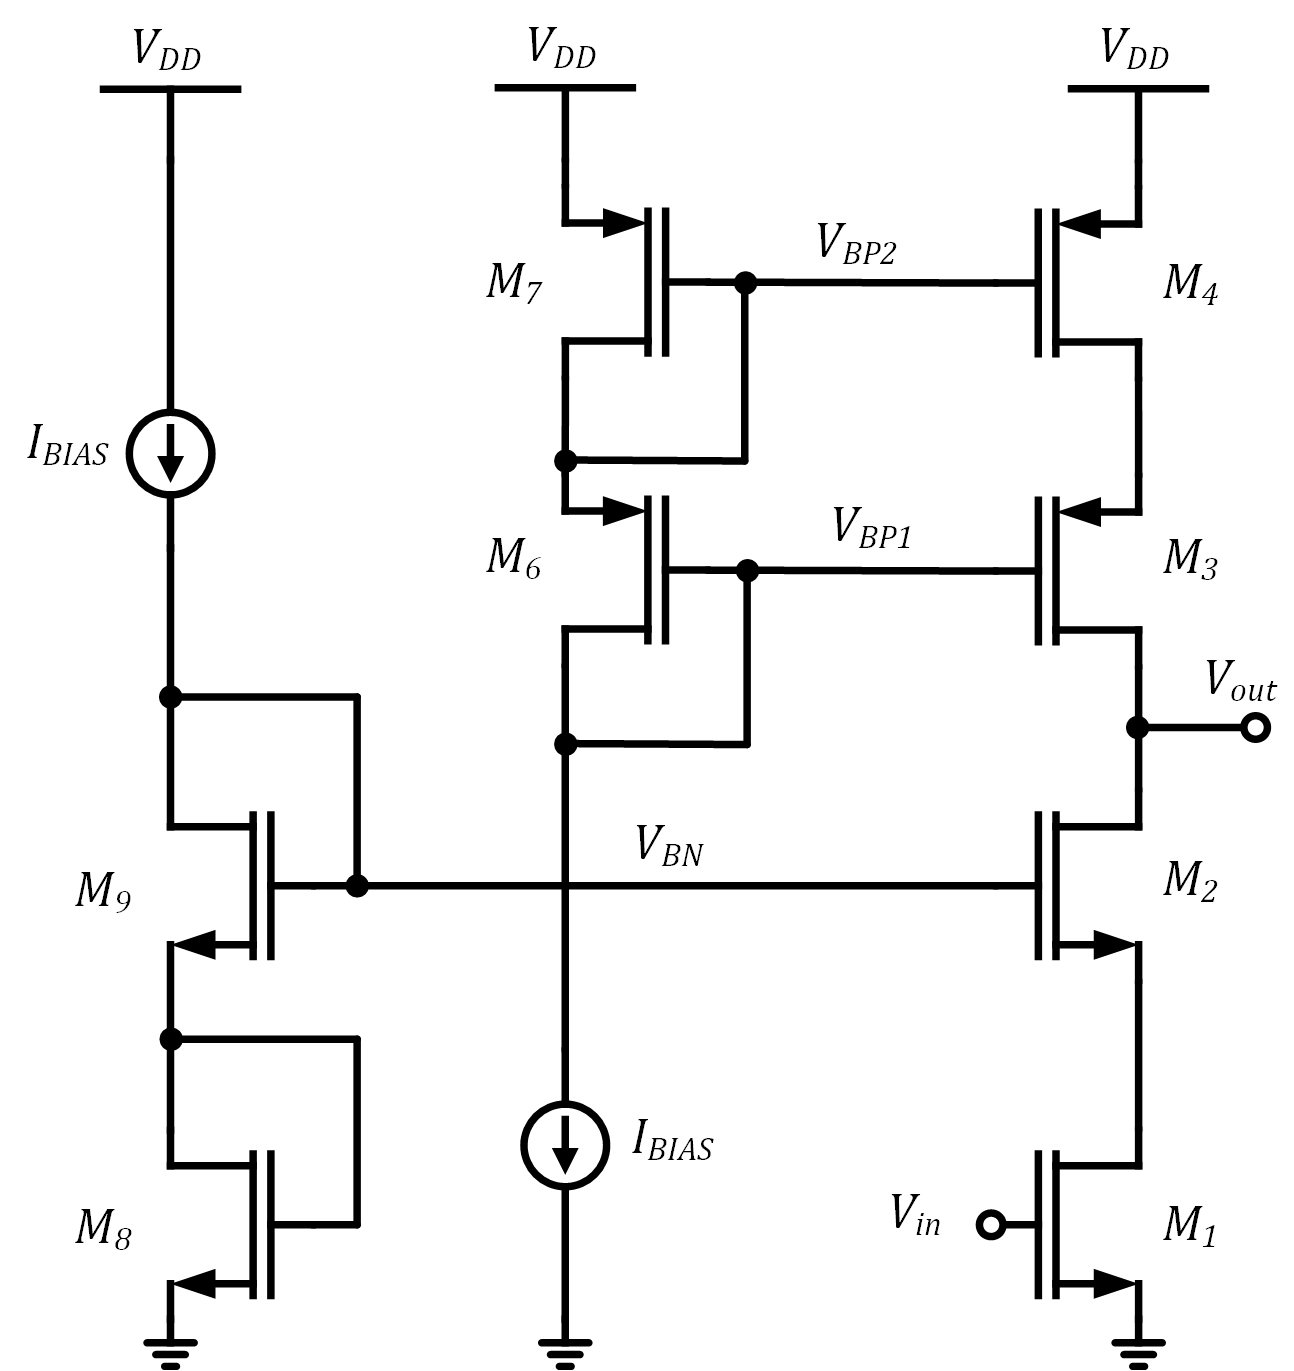
\includegraphics{cascode_biasing.png}
\caption{cascode\_biasing.png}
\end{figure}

    \begin{itemize}
\tightlist
\item
  Here is one possible bias configuration (of several) for a cascode
  amplifier
\item
  A cascode current mirror (\(M_{3,4}, M_{6,7}\)) is used to set the
  bias voltages \(V_{BP1}\) and \(V_{BP2}\)
\item
  \(V_{BN}\) establishes a gate voltage for \(M_2\), while a
  diode-connected \(M_8\) ensures that \(M_2\)'s source is at a high
  enough potential to keep \(M_1\) in saturation
\end{itemize}

    \hypertarget{cascode-voltage-swing}{%
\subsection{Cascode voltage swing}\label{cascode-voltage-swing}}

    \begin{figure}
\centering
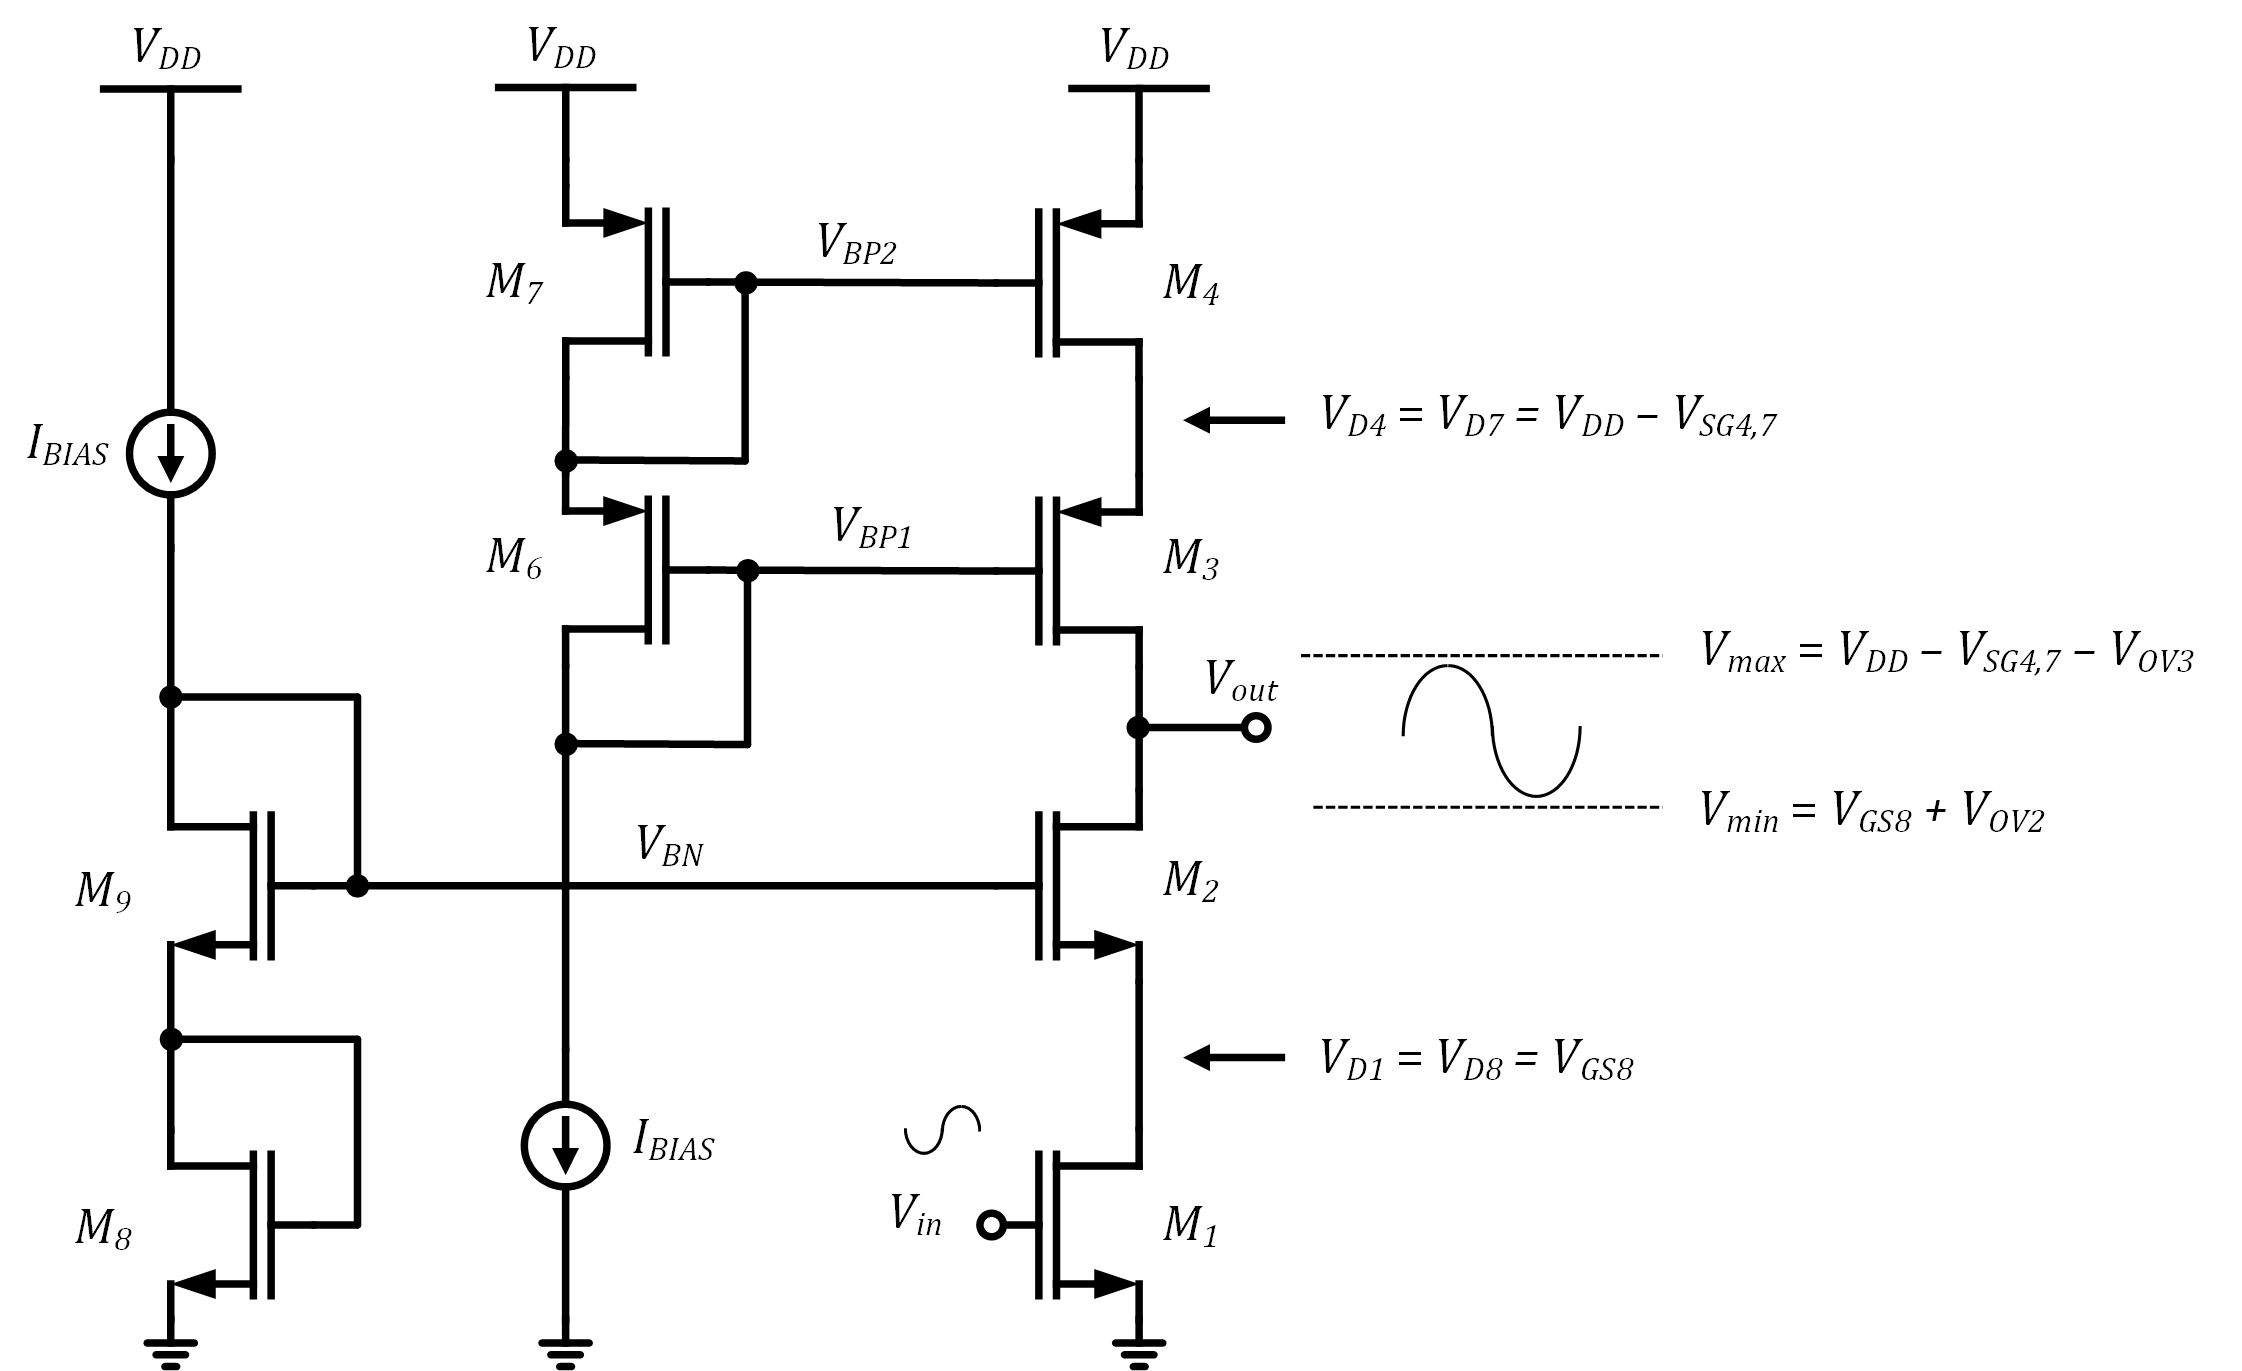
\includegraphics{cascode_amplifier_swing.png}
\caption{cascode\_amplifier\_swing.png}
\end{figure}

    \hypertarget{summary}{%
\subsection{Summary}\label{summary}}

    \begin{itemize}
\tightlist
\item
  Degeneration and cascoding use negative feedback to signficantly
  increase the output resistance of the simple current source
\item
  Higher output resistance means greater precision in current mirrors,
  and higher gain in amplifiers
\item
  Adding a cascode transistor also increases the output resistance of
  the input path
\item
  The gain of the cascode amplifier is approximately \(g_{m}r_o\) times
  higher than that of a common-source amplifier with active load
\item
  Device stacking also results in the body effect, which should be
  considered during design
\item
  The increased output resistance comes at the cost of lower output
  swing, due to stacking of more transistors
\end{itemize}


    % Add a bibliography block to the postdoc
    
    
    
\end{document}
